%\begin{figure}[H]
%    \centering
%    \includegraphics[width=\textwidth]{imagenes/passwdfile.png}
%    \vspace{10pt}
%    \footnotesize{Fuente: https://...}
%\end{figure}

% \begin{figure}[H]
%     \centering 
% 	\begin{subfigure}[t]{0.48\textwidth}
% 	    \centering
% 	    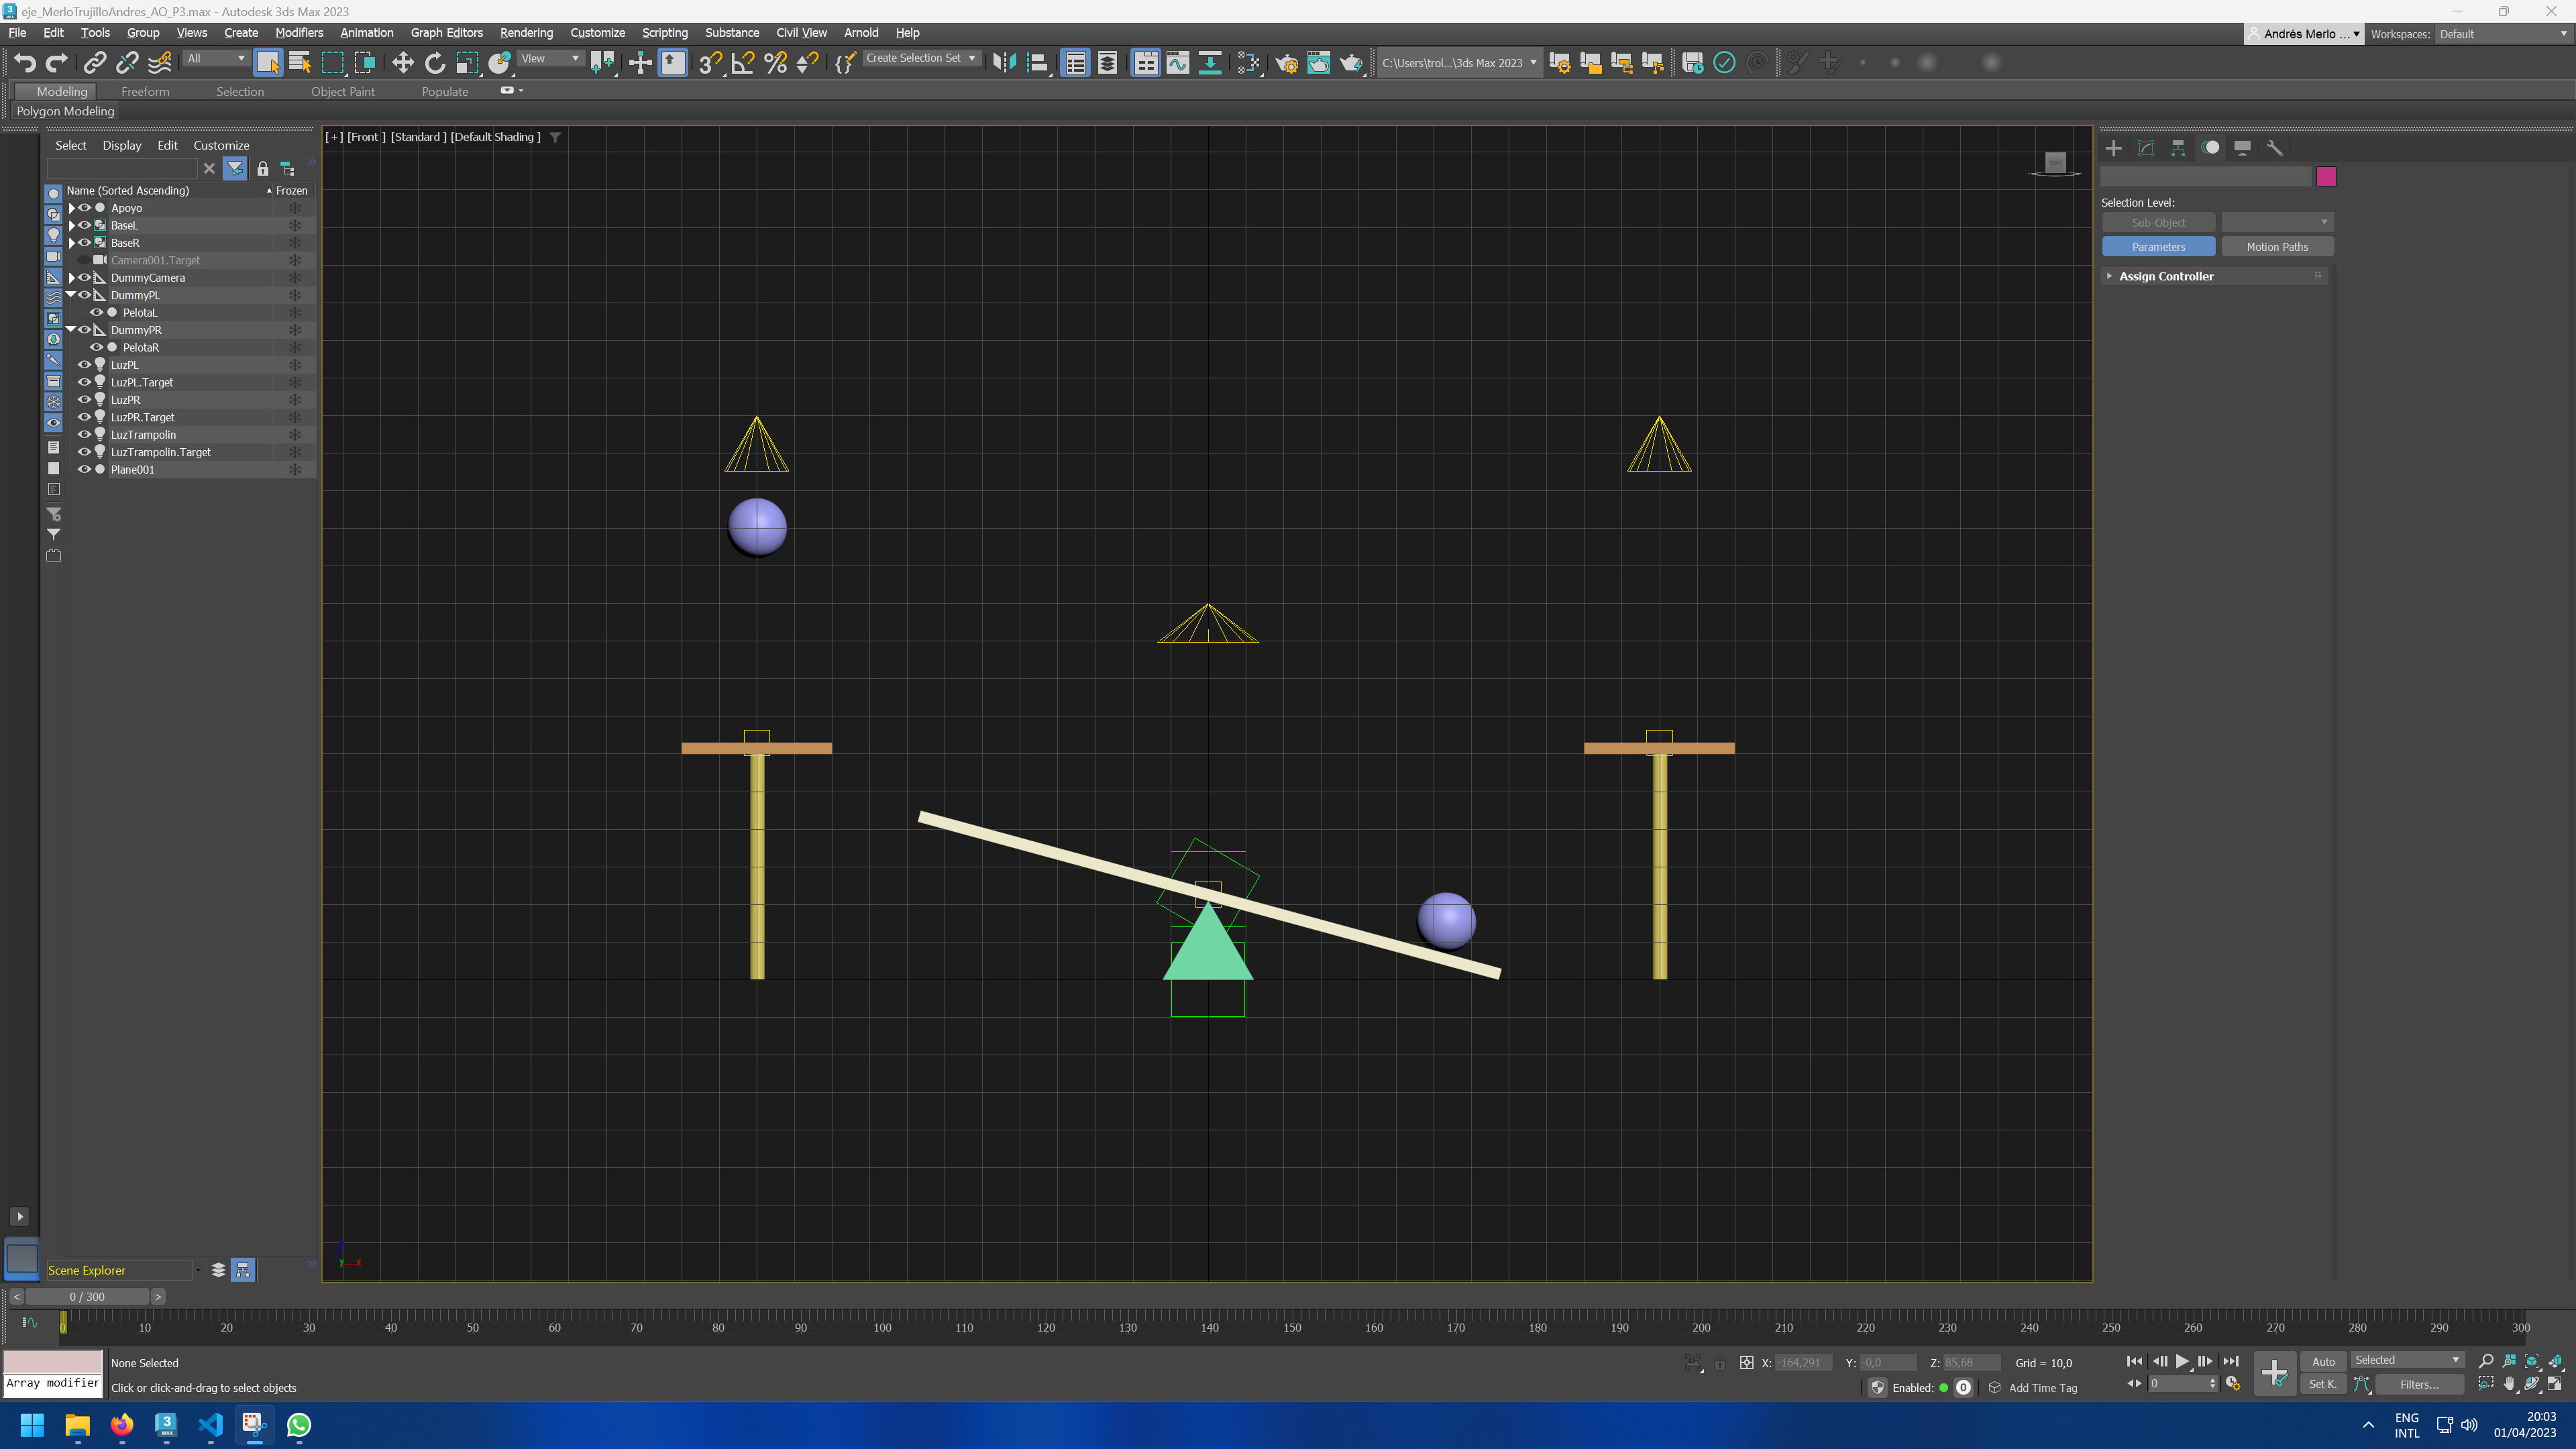
\includegraphics[width=\textwidth]{imagenes/Ejercicio 1/keyframes/0.png}
%         \caption{Pelotas en el instante 0.}
%     \end{subfigure}
%     \hfill
%     %\par\bigskip %si se desea dejar un margen entre la imagen de arriba y de abajo
% 	\begin{subfigure}[t]{0.48\textwidth}
% 	    \centering
% 	    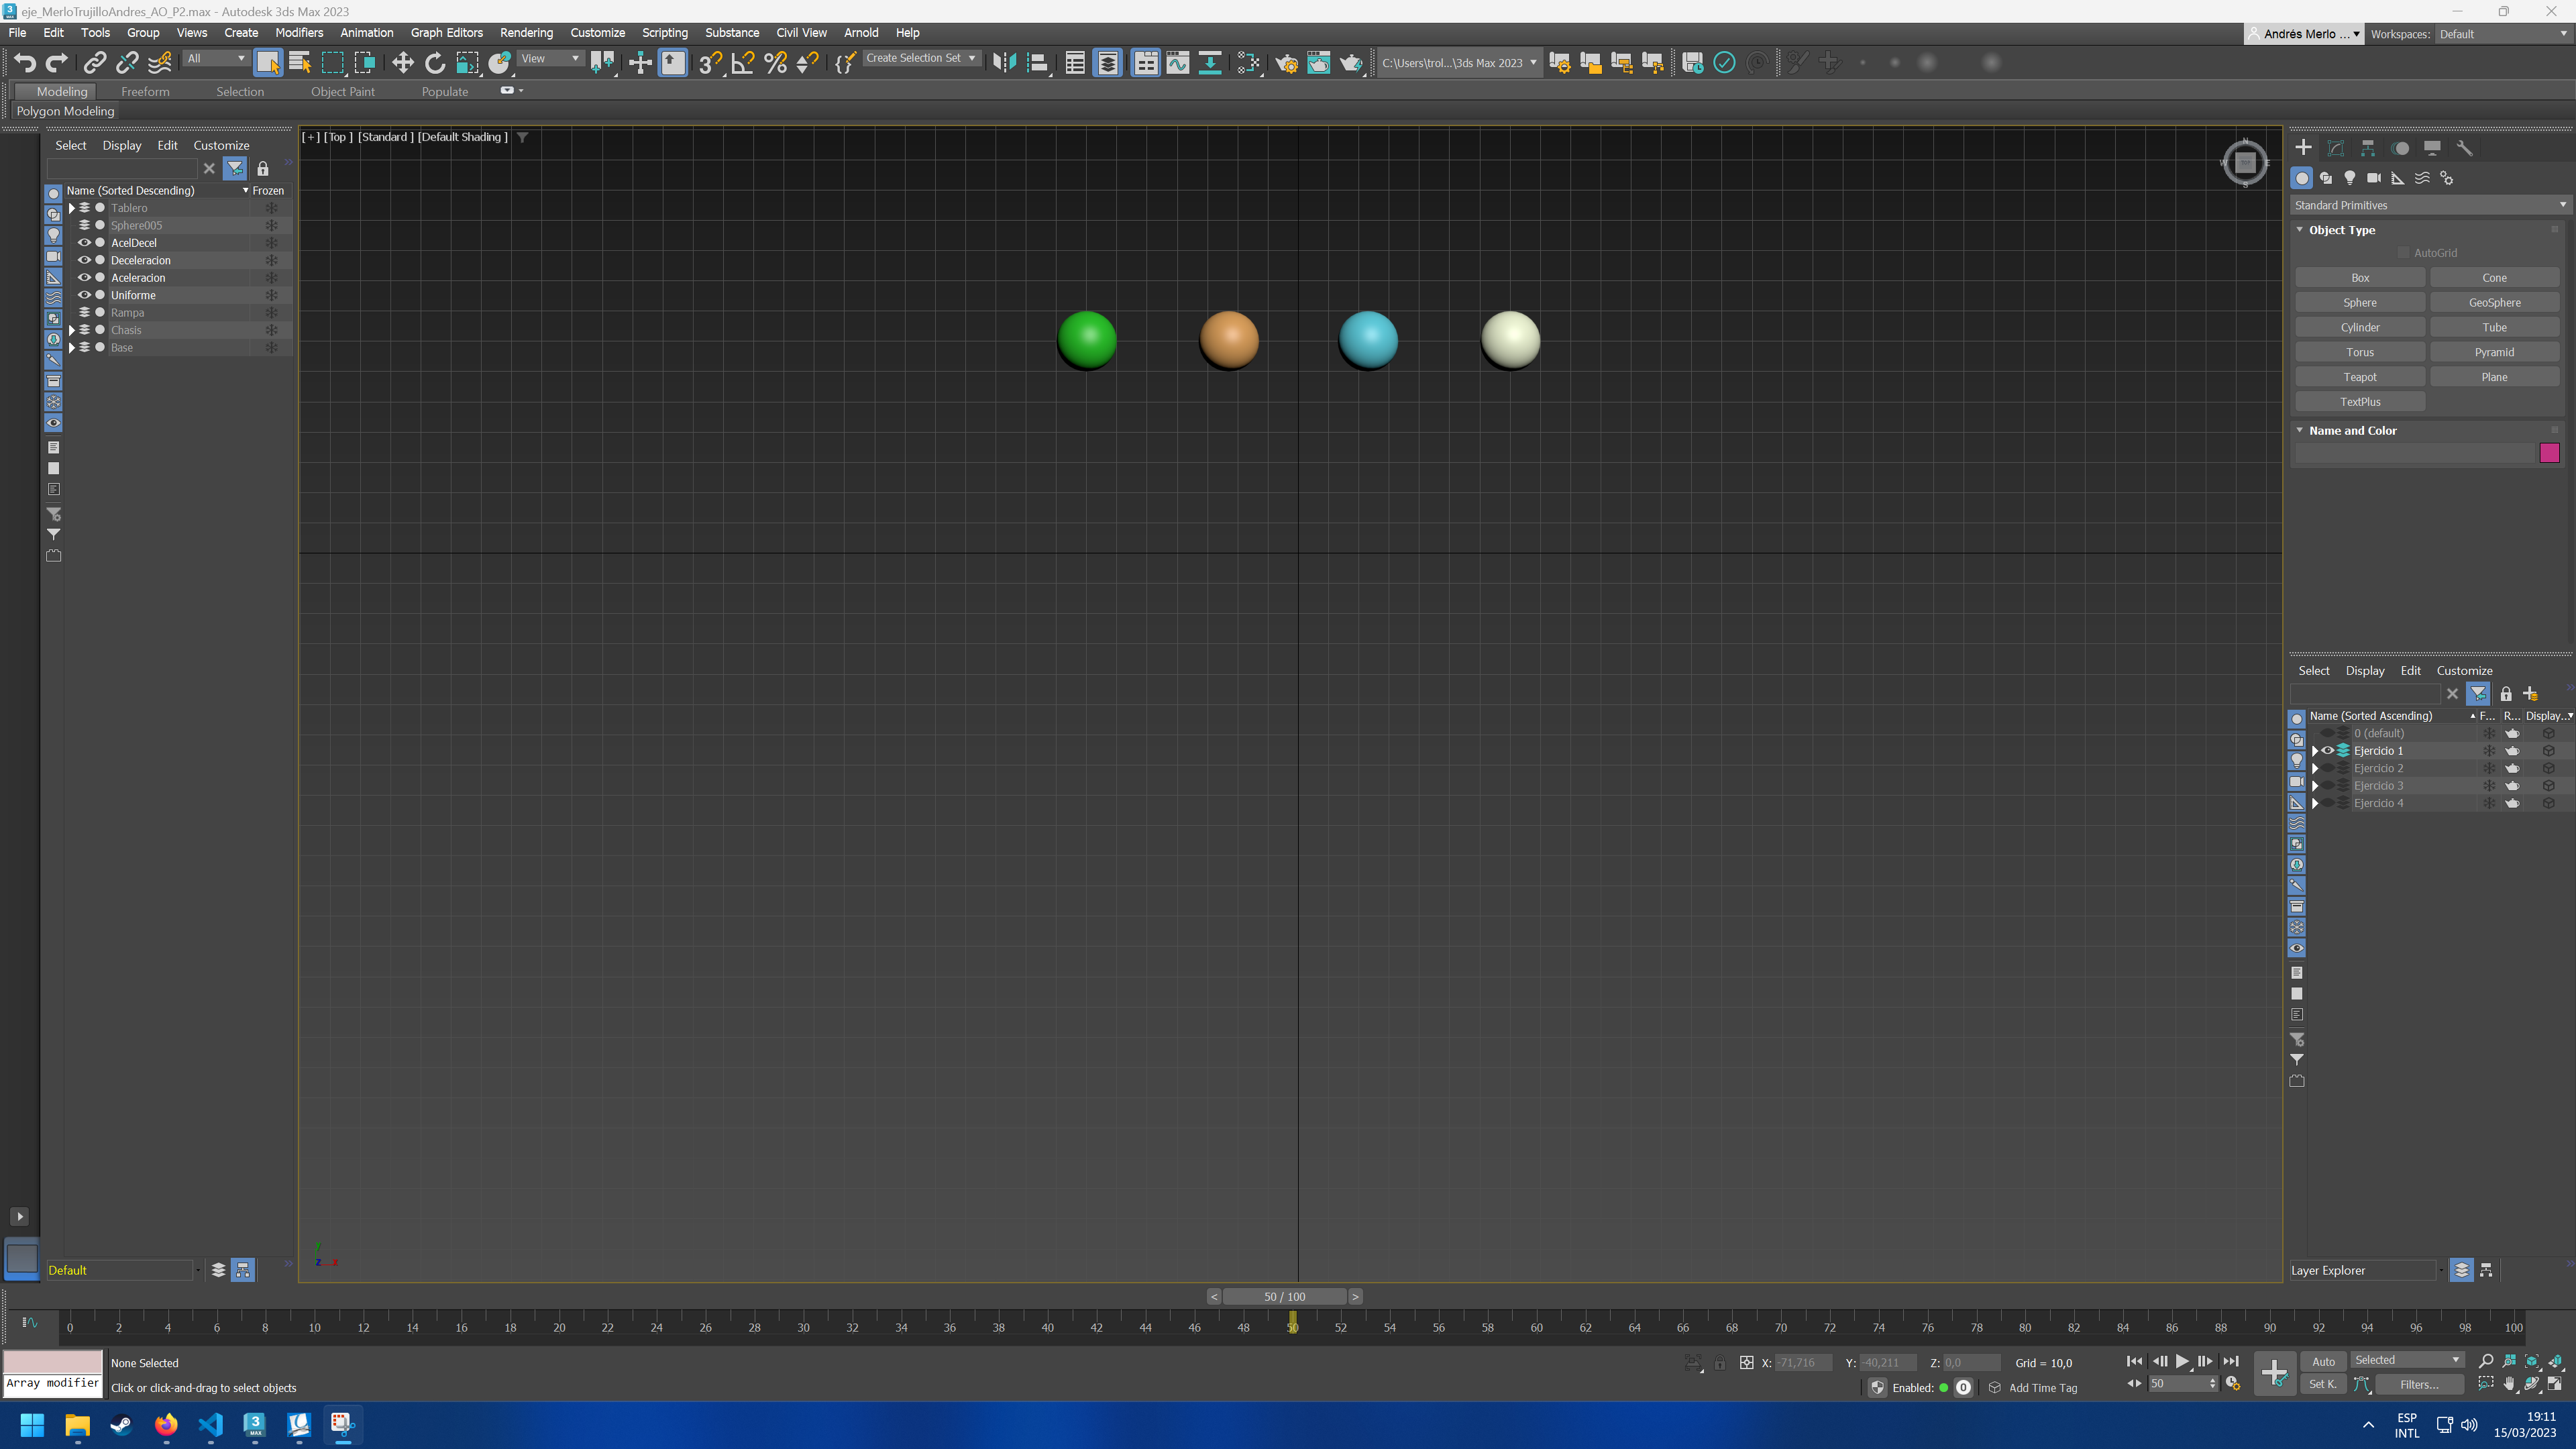
\includegraphics[width=\textwidth]{imagenes/Ejercicio 1/keyframes/50.png}
%         \caption{Pelotas en el instante 50.}
%     \end{subfigure}    
% \end{figure}

\section{Animación de la escena}

La animación la he realizado algo distinta a la que se pedía en el guion, ya que le comenté al profesor que el resultado final era muy lento y me dijo que podía añadir algunos rebotes antes de comenzar la animación pedida. Para dar simetría, he animado dos rebotes al principio de la animación y al final y en ambas pelotas, para que la repetición inversa sea igual. 

\bigskip

Además, se pide hacer que los últimos 5 segundos realice la misma animación, pero al revés. Esto se realiza usando la forma ping-pong, accesible desde la ventana para el editor de curvas.

\begin{figure}[H]
   \centering
   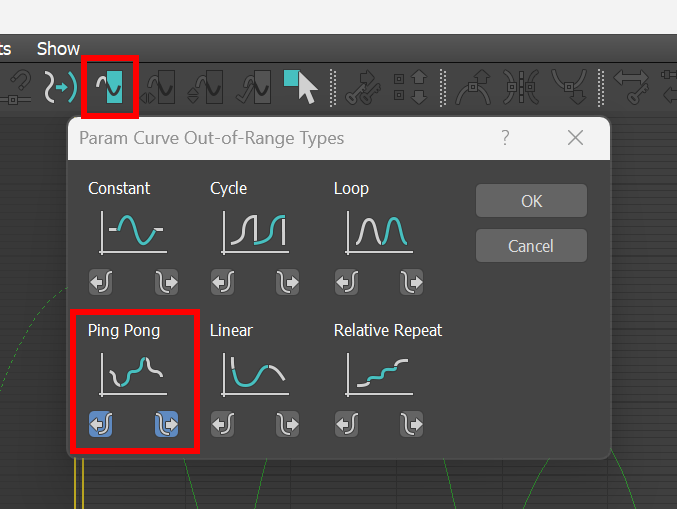
\includegraphics[width=0.5\textwidth]{imagenes/misc/ping-pong.png}
   \caption{Pasos necesarios para seleccionar el tipo ping-pong.}
\end{figure}

Esta forma obliga a repetir \textit{keyframes} en los instantes 0 y 150; es decir, no va a haber cambio con el \textit{keyframe} siguiente o anterior. Esto es necesario porque hay animaciones que no duran lo mismo, como el trampolín, que su animación es más corta y si no se hiciera daría como resultado un giro prematuro, haciendo que la animación no sea correcta en los últimos 5 segundos.

\bigskip

Para animar el movimiento del trampolín, he movido el pivote de la plataforma que oscila hacia el punto que toca con el punto de apoyo, de forma que gire de manera realista.

% foto del trampolin
\begin{figure}[H]
   \centering
   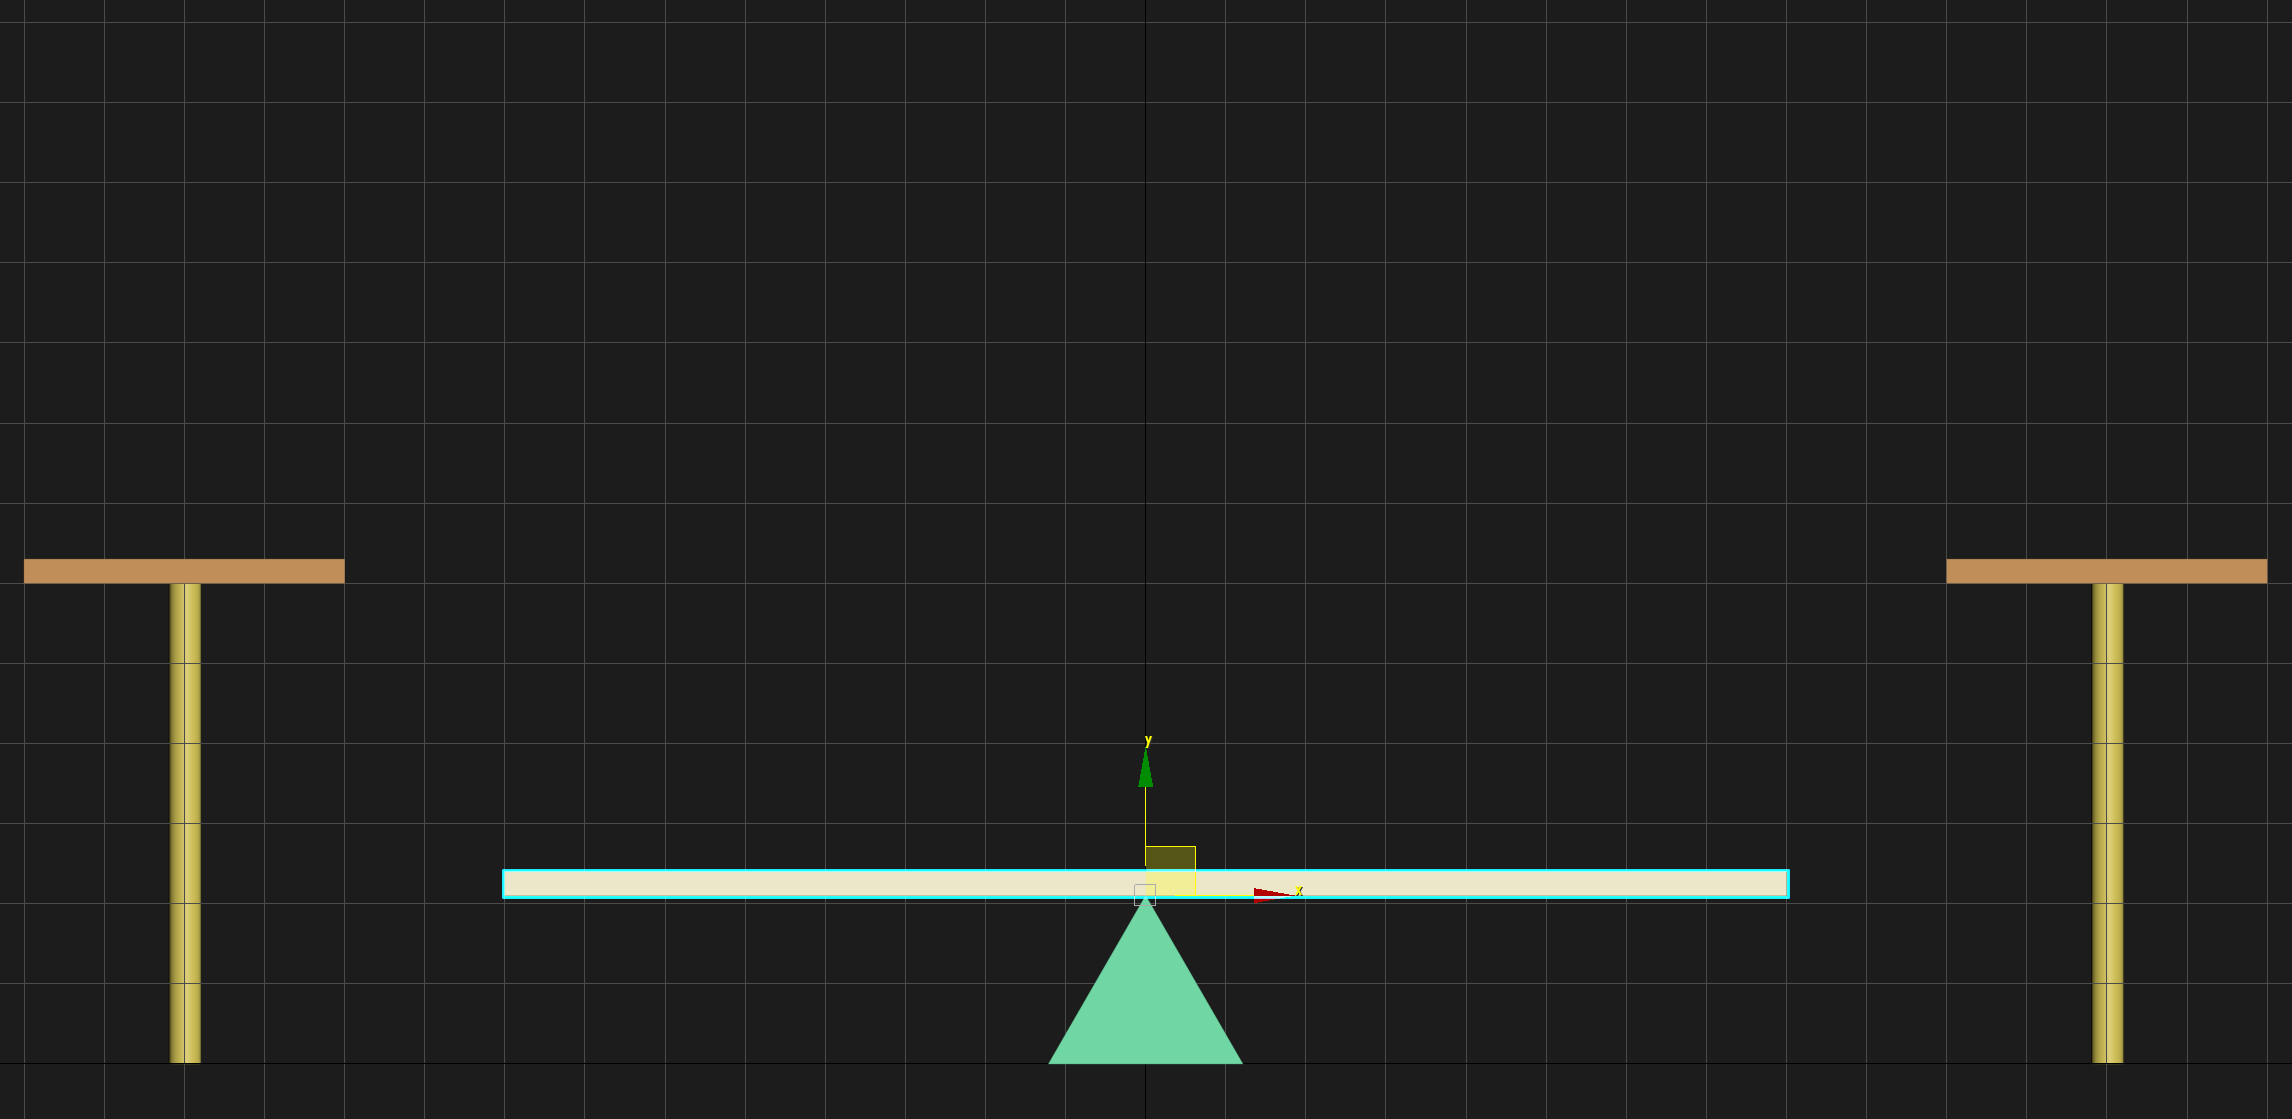
\includegraphics[width=0.7\textwidth]{imagenes/misc/PivotTrampolin.png}
   \caption{Pivote de la plataforma del trampolín.}
\end{figure}

% rescribir
Para animar el movimiento de las pelotas, he usado un objeto \textit{Dummy} con centro en la superficie donde tocan las pelotas el balancín y centrado en el eje X. Este objeto será padre de las pelotas en la jerarquía.

\begin{figure}[H]
    \centering 
	\begin{subfigure}[t]{0.48\textwidth}
	    \centering
	    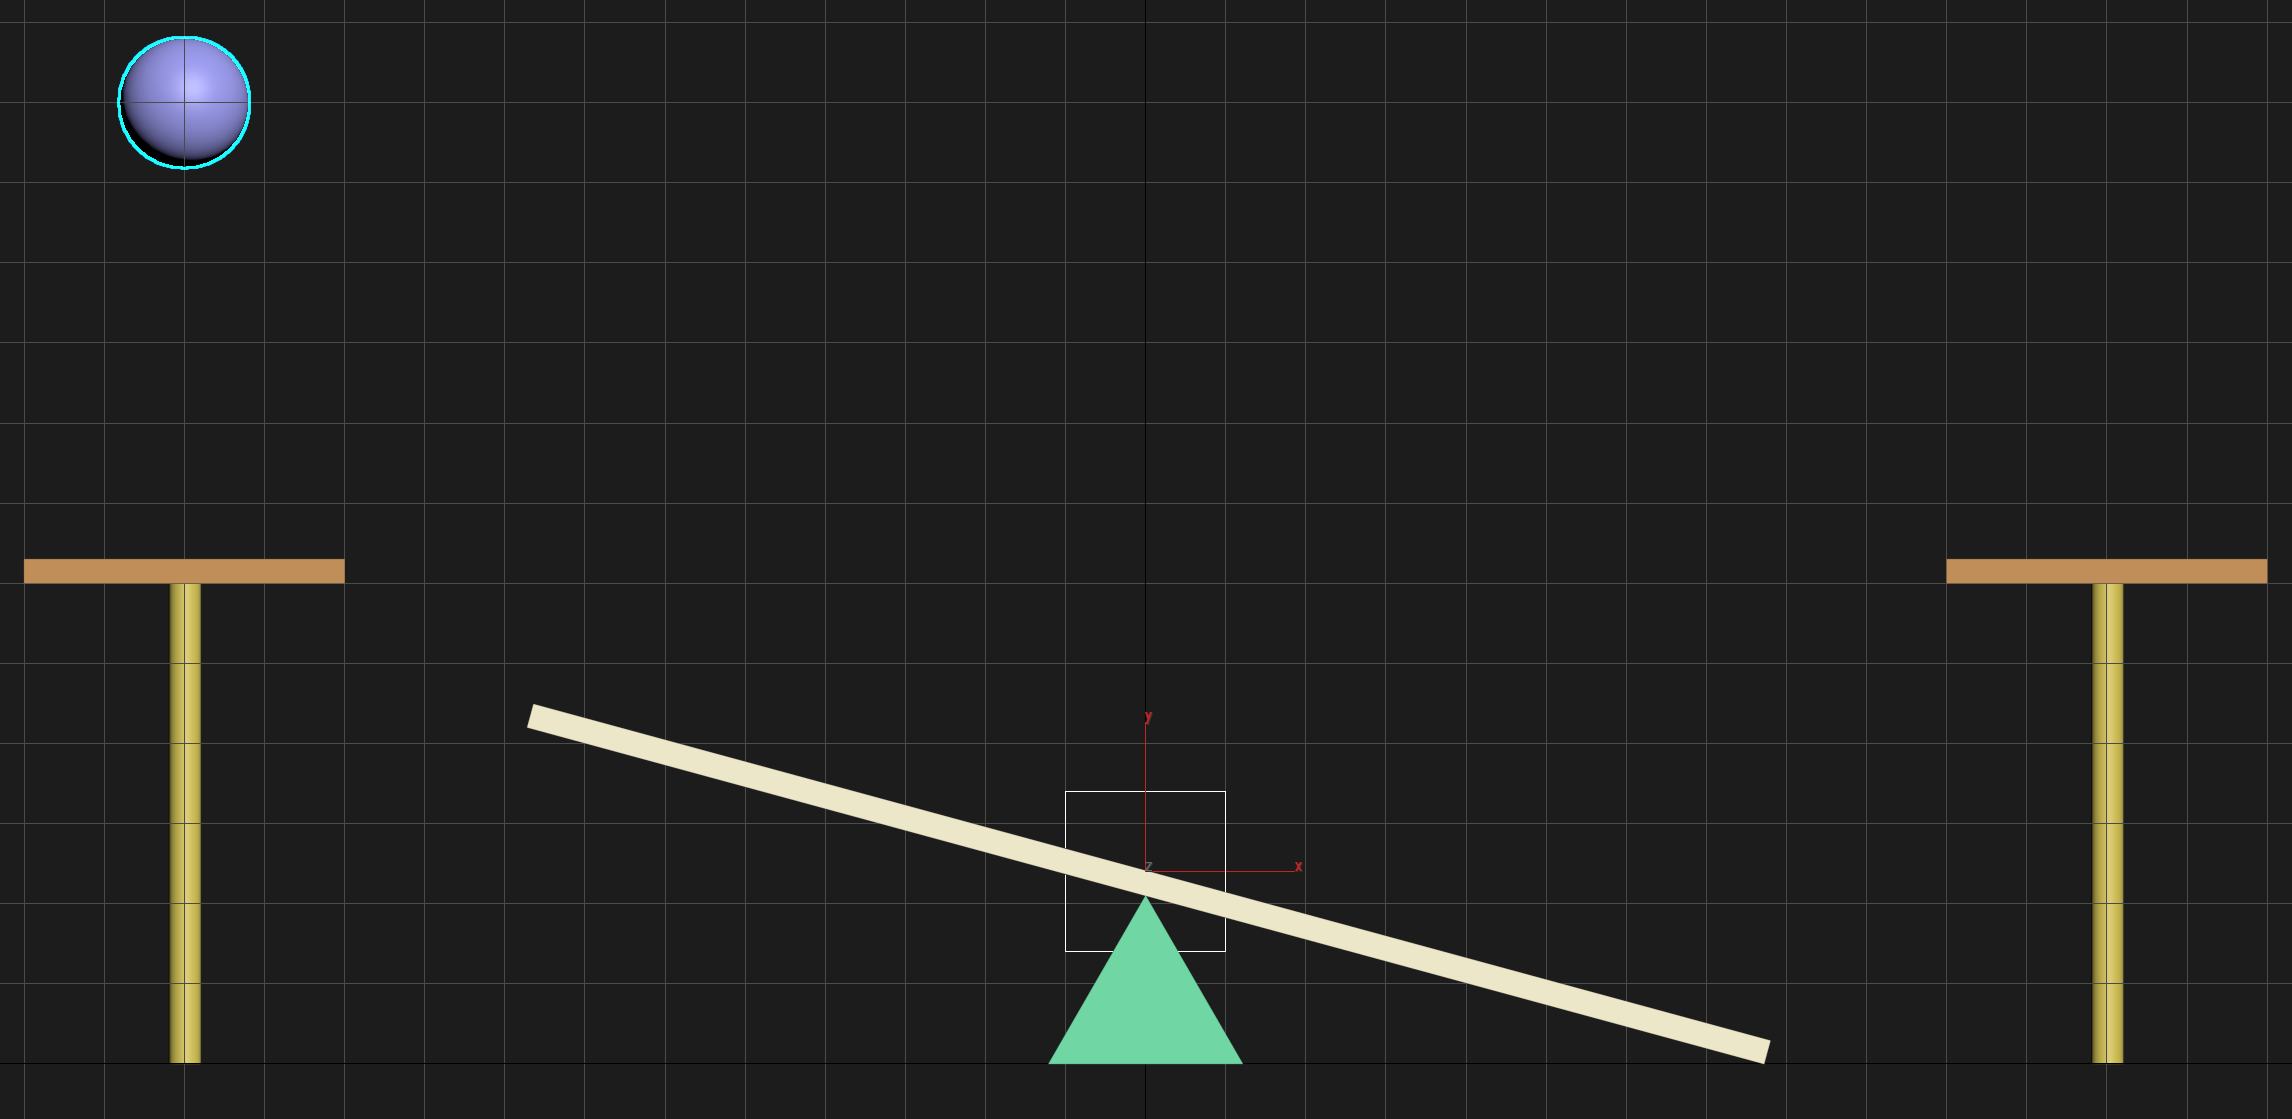
\includegraphics[width=\textwidth]{imagenes/misc/PLDummy.png}
   \caption{Pelota izquierda junto a su \textit{Dummy}.}
    \end{subfigure}
    \hfill
    %\par\bigskip %si se desea dejar un margen entre la imagen de arriba y de abajo
	\begin{subfigure}[t]{0.48\textwidth}
	    \centering
       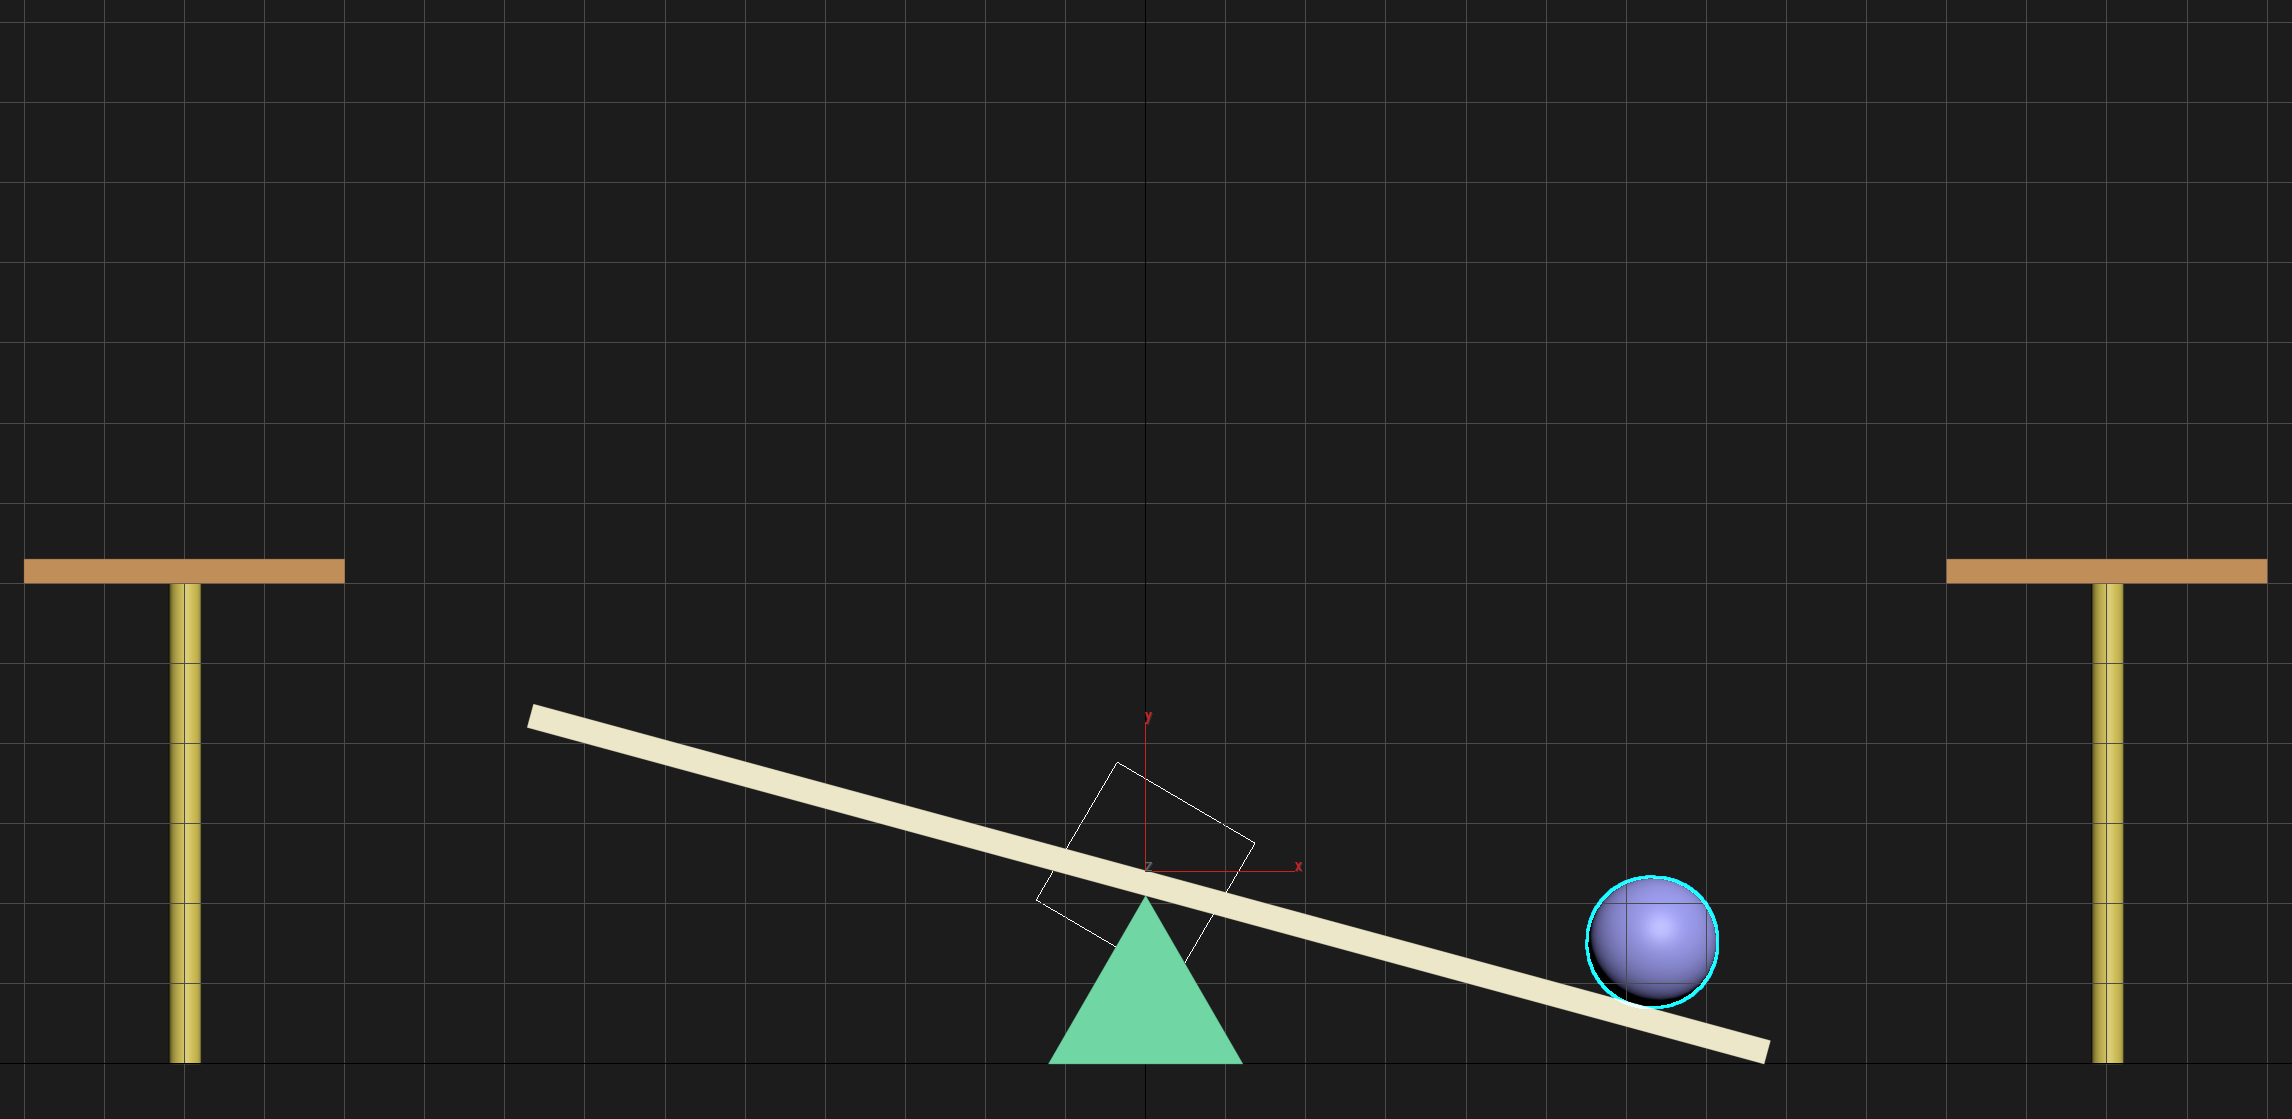
\includegraphics[width=\textwidth]{imagenes/misc/PRDummy.png}
   \caption{Pelota derecha junto a su \textit{Dummy}.}
    \end{subfigure}    
    \caption{\textit{Dummies} utilizados para realizar la animación de las pelotas en el trampolín.}
\end{figure}




\bigskip

Asimismo, para que la trayectoria que realicen no se vea afectada por la rotación del \textit{Dummy}, este se debe encontrar sin ninguna rotación en el momento en el que salen/entran al trampolín. Si no se siguiera esto, la trayectoria seguida en los saltos estaría rotada, de acuerdo al ángulo que tenga el \textit{Dummy} en ese momento.

\bigskip

% Ahora bien, como puede haber confusión sobre los distintos \textit{keyframes} para los objetos de la escena, voy a dividir cada objeto junto a su \textit{Dummy}, si lo tiene, en subsecciones:

Voy a dividir cada parte de la escena animada en subsecciones, que se encuentran a continuación.

\subsection{Pelota de la izquierda}
Como he dicho anteriormente, la animación de la pelota de la izquierda consiste en utilizar una jerarquía, cuyo padre sea un \textit{Dummy} centrado en el trampolín, para realizar el balanceo del mismo cuando se mueve.

\bigskip

Por tanto, los \textit{keyframes} para la pelota de la izquierda son:

\begin{itemize}
    \item \textbf{Instante 0: }La pelota se encuentra sobre su base, a cierta altura de la misma para realizar varios rebotes.
    \item \textbf{Instante 14: }La pelota se encuentra tocando la superficie de la base, debido a la caída de la pelota.
    \item \textbf{Instante 26: }La pelota se encuentra en el aire, con la misma altura que en el instante 0. No disminuyo la altura del rebote para que la animación ping-pong funcione de manera más o menos realista.
    \item \textbf{Instante 38: }La pelota se encuentra sobre la superficie de la base, esta vez lista para saltar al trampolín.
    \item \textbf{Instante 48: }La pelota se encuentra en su punto más alto del salto hacia el trampolín.
    \item \textbf{Instante 58: }La pelota ha caído y se encuentra sobre el trampolín.
    \item \textbf{Instante 150: }Exactamente igual que el instante anterior, para que la animación se pueda repetir correctamente.
\end{itemize}

\bigskip

Las curvas de animación para la pelota son:

\begin{figure}[H]
   \centering
   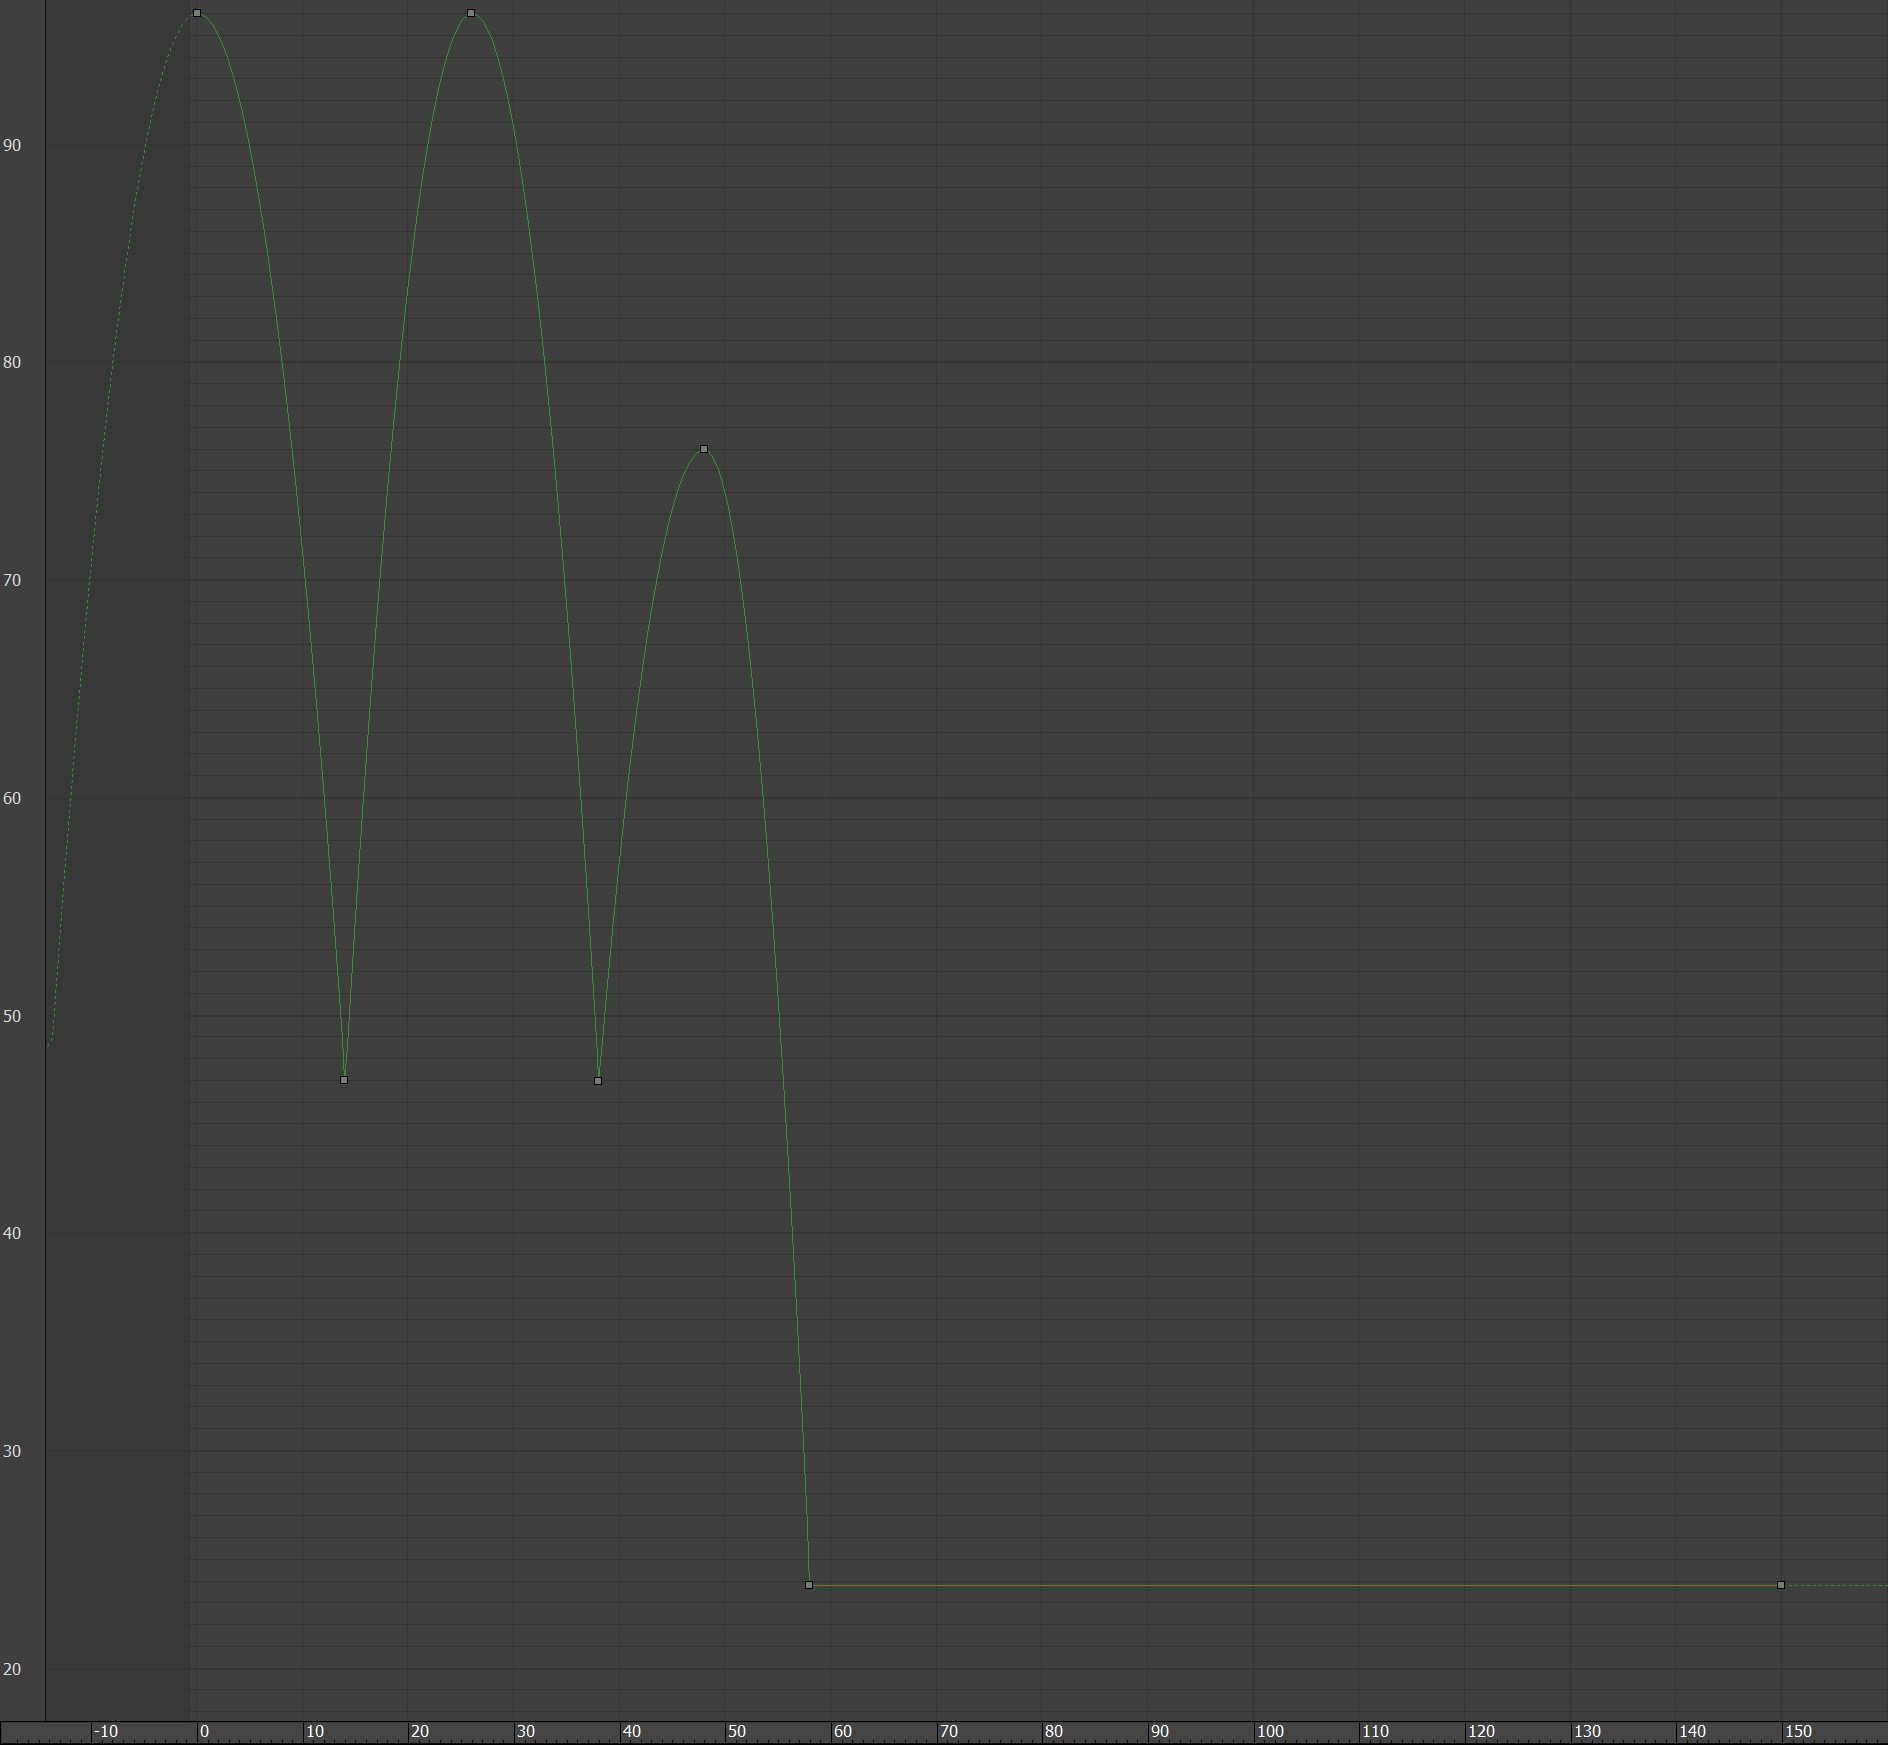
\includegraphics[width=0.6\textwidth]{imagenes/curvas/PL/pelota/green.png}
   \caption{Curva que representa la posición en el eje Y de la pelota con respecto el tiempo.}
\end{figure}

Esta curva representa la posición en el eje Y de la pelota con respecto el tiempo. Realmente se ve reflejado en un cambio en el eje Z en coordenadas del mundo, pero a causa de usar los \textit{dummies}, este eje cambia. Sabiendo esto, se puede ver como la curva realiza una forma parabólica, simulando los efectos que tiene la gravedad sobre la pelota para acelerarla en la bajada y desacelerarla en la subida. Finalmente se queda parada sobre el trampolín y dicho estado se extiende hasta el instante 150, para que la animación inversa funcione.

\begin{figure}[H]
   \centering
   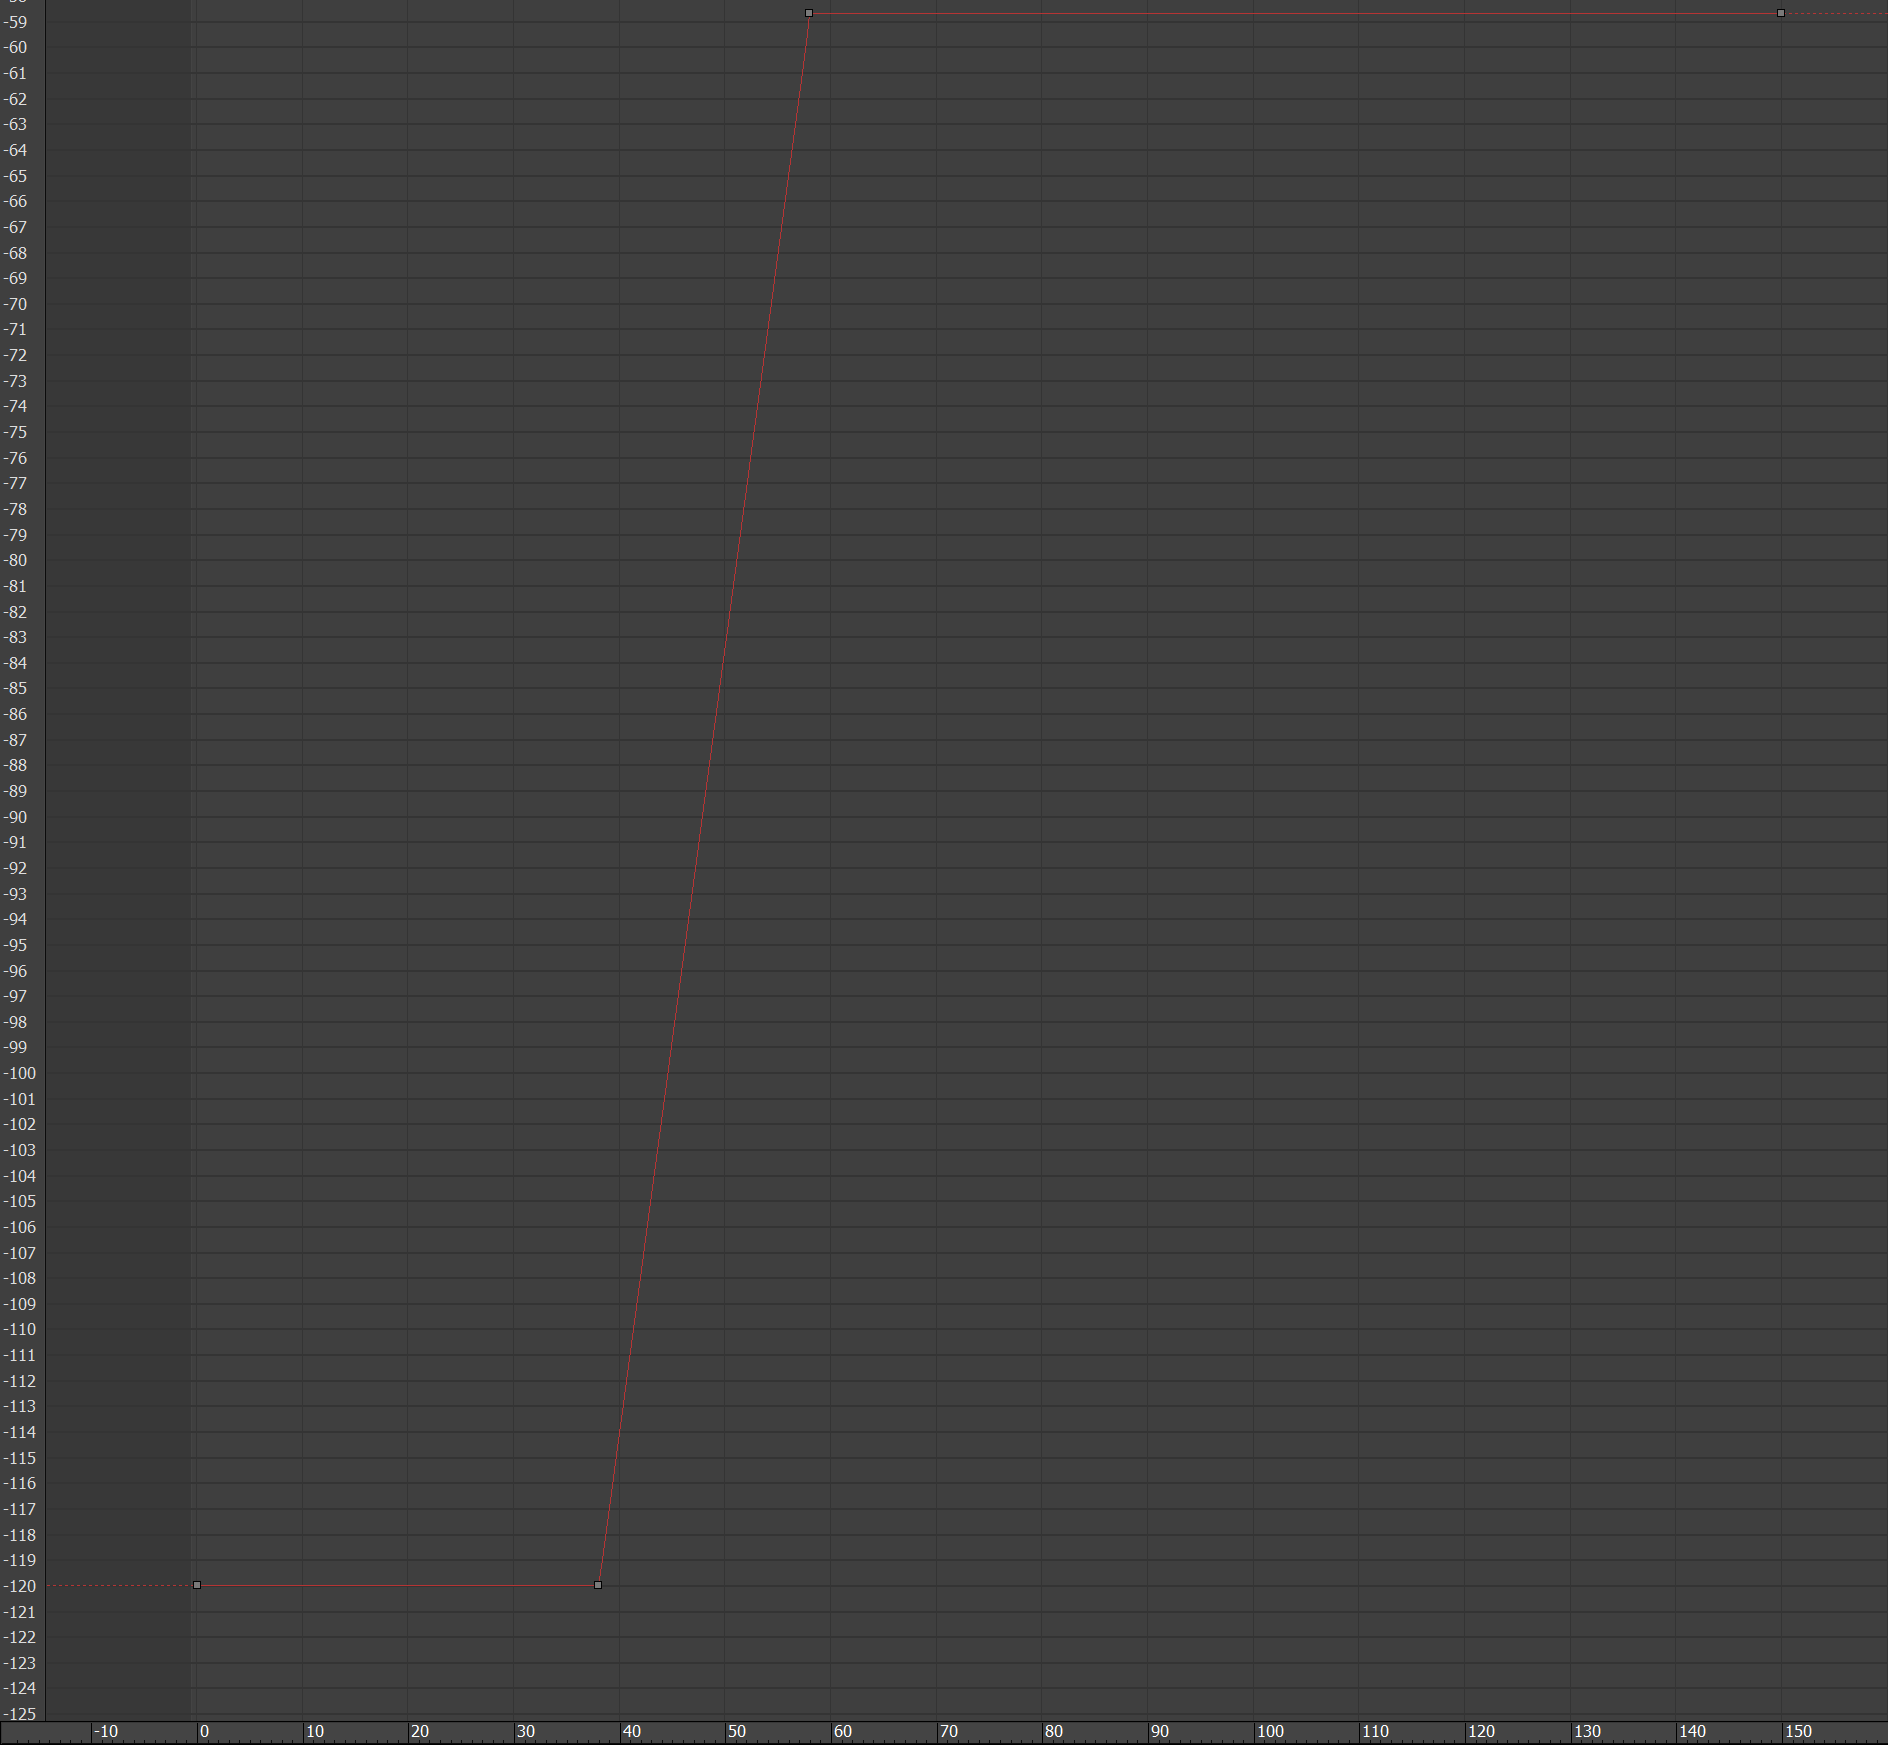
\includegraphics[width=0.6\textwidth]{imagenes/curvas/PL/pelota/red.png}
   \caption{Curva que representa la posición en el eje X con respecto el tiempo.}
\end{figure}

% rescribir
Esta curva representa la posición en el eje X con respecto el tiempo, solo desde la posición de la base hasta en el momento que toca por primera vez el trampolín, ya que las siguientes animaciones las realiza el \textit{Dummy} correspondiente. He elegido una función lineal porque es la que me ha parecido más realista de todas las opciones, dentro de lo que cabe. 

\bigskip

Los \textit{keyframes} para el \textit{Dummy} de la pelota de la izquierda son:

\begin{itemize}
    \item \textbf{Instante 0: }Se encuentra en su posición inicial, sin ninguna rotación para hacer que la trayectoria de la pelota sea correcta. Se hace para que la animación inversa funcione de manera correcta.
    \item \textbf{Instante 58: }Exactamente igual que el anterior \textit{keyframe}.
    \item \textbf{Instante 92: }El \textit{Dummy} se encuentra rotado hacia la izquierda, para animar el balanceo del balancín de manera correcta.
    \item \textbf{Instante 150: }Exactamente igual que el instante anterior, se hace para que la animación ping-pong comience al unísono con las demás.
\end{itemize}

\newpage

Las curva de animación para el \textit{Dummy} son:

\begin{figure}[H]
    \centering
    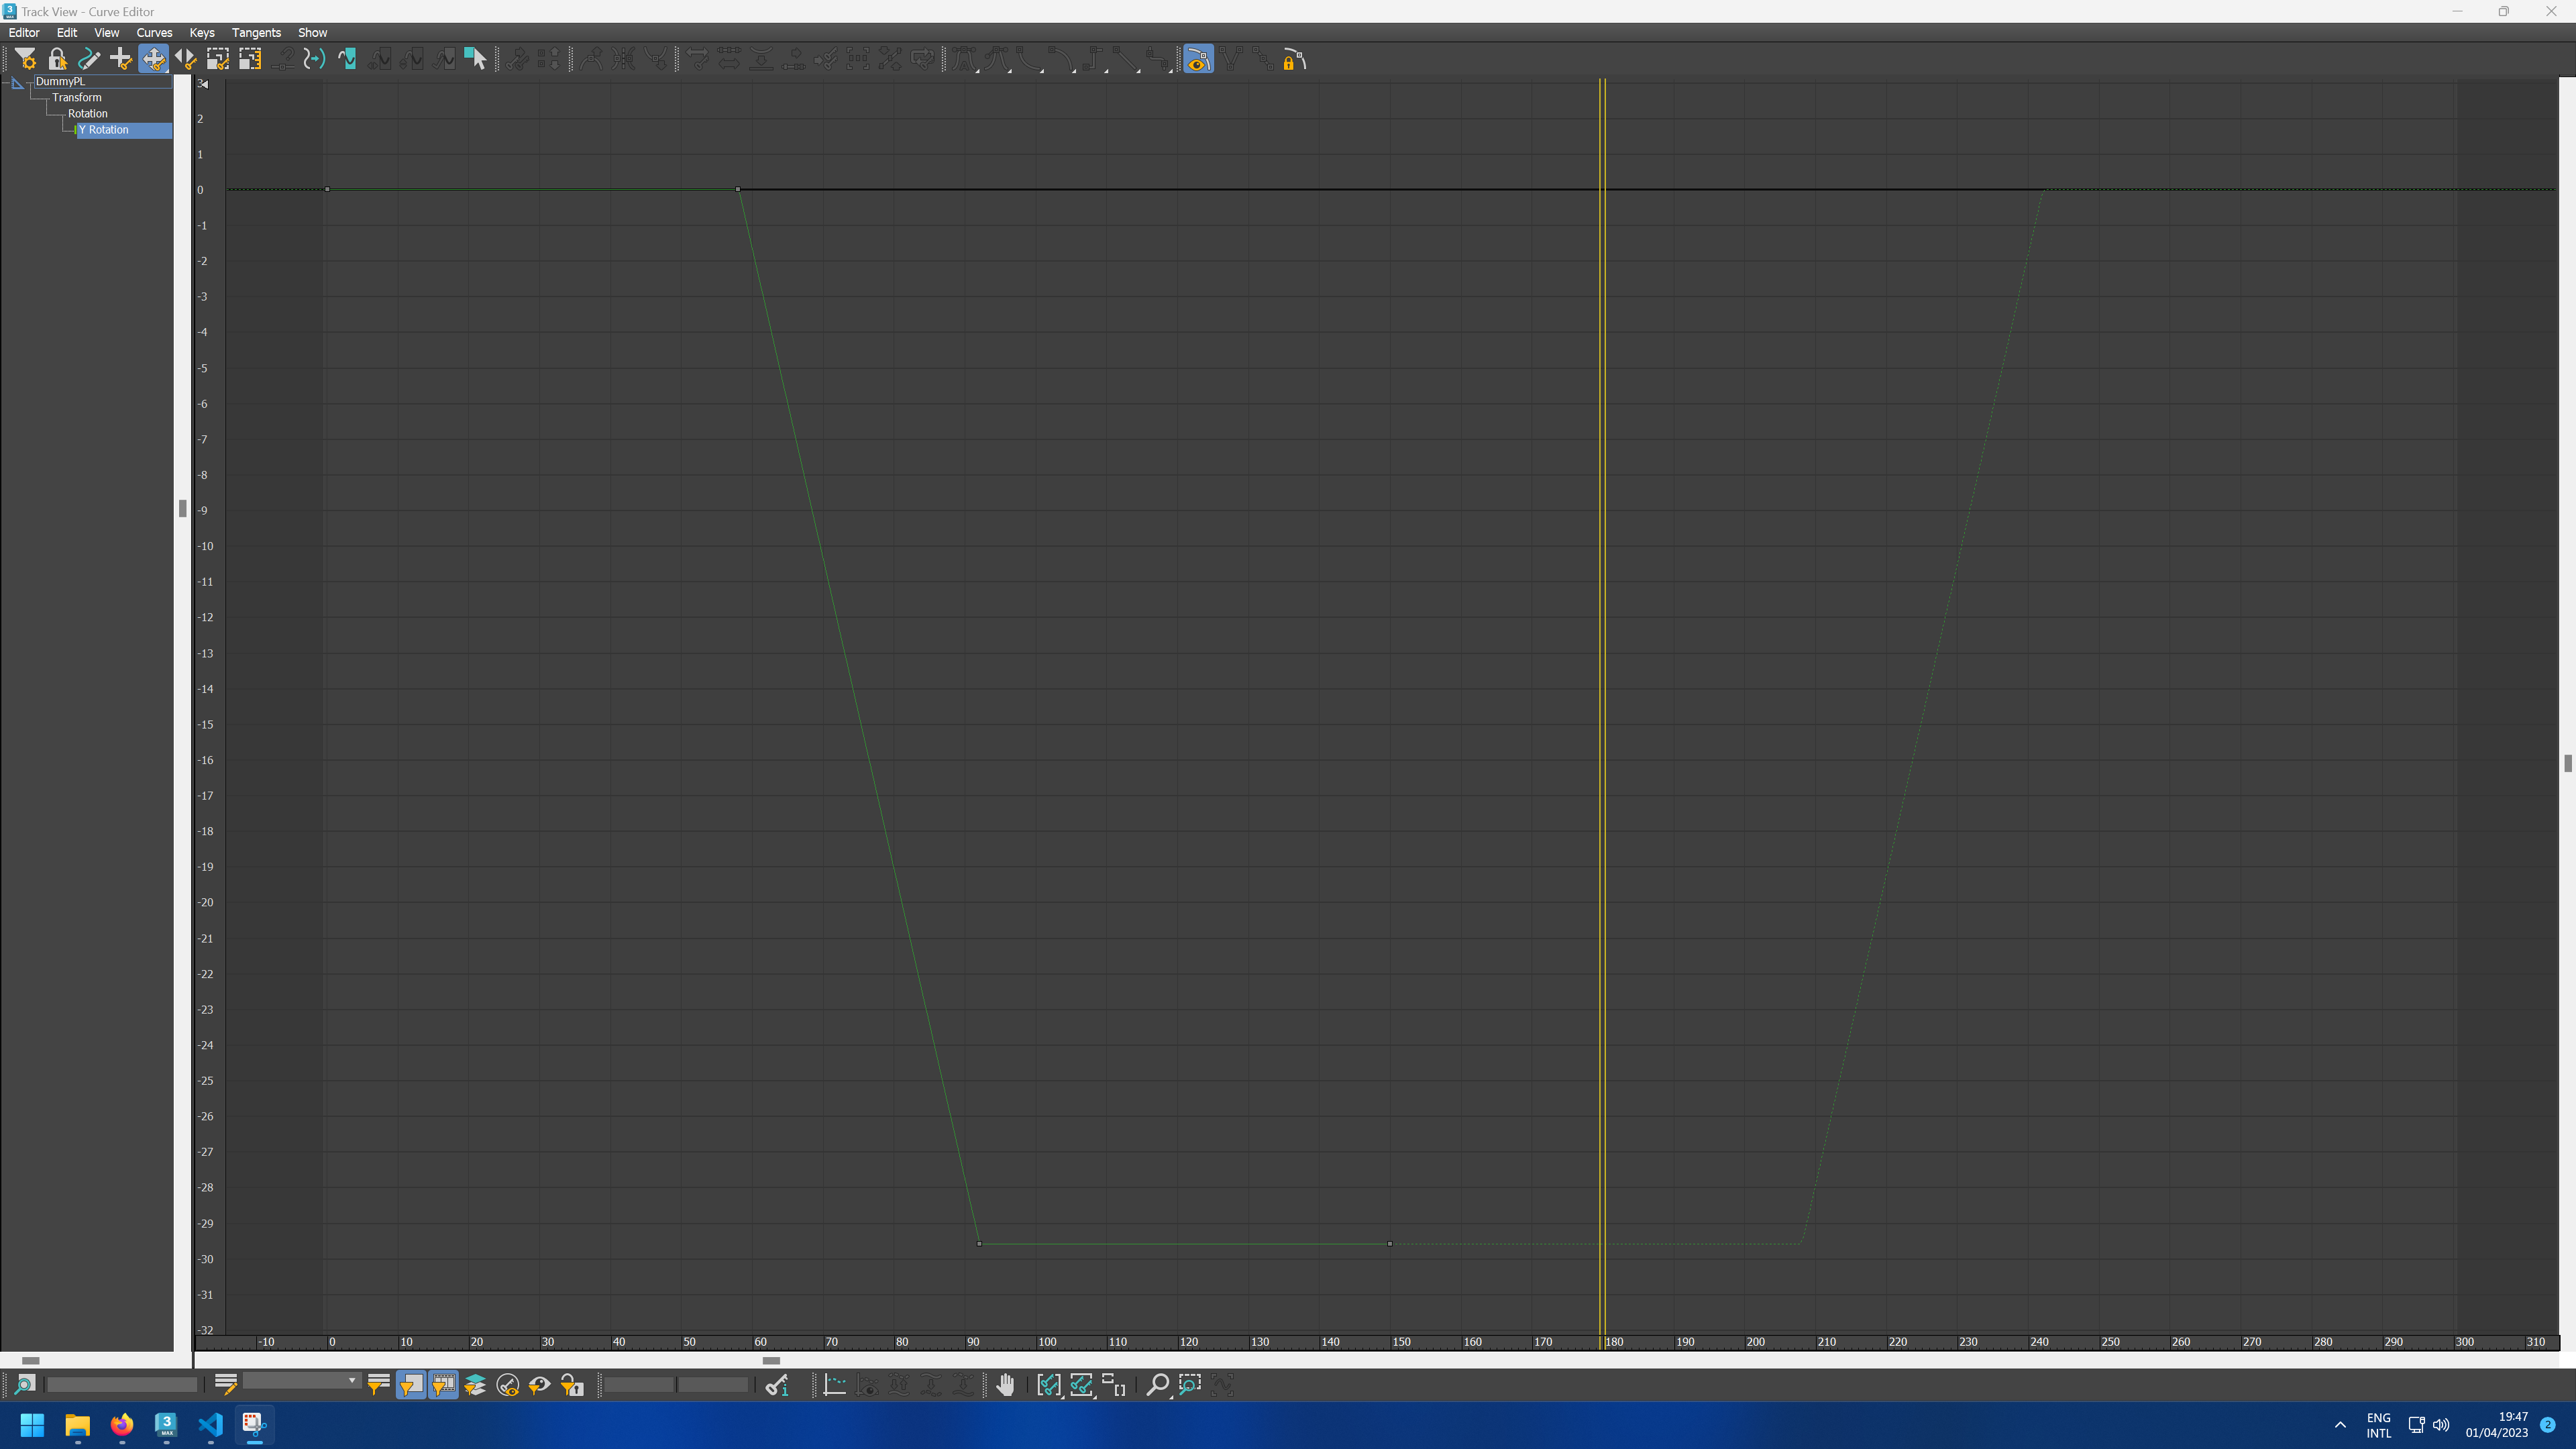
\includegraphics[width=0.6\textwidth]{imagenes/curvas/PL/dummy/green.png}
    \caption{Curva que representa la rotación en el eje Y con respecto el tiempo.}
 \end{figure}

 % rescribir, muy repetido trampolín y pelota
% Esta curva representa la rotación del \textit{dummy} con respecto al tiempo. La he animado de forma lineal porque, al seguir la animación del trampolín, esta debe seguirla también; es decir, como la energía potencial que tiene la pelota se le transfiere al trampolín, haciendo que el trampolín tenga la misma velocidad que la que tenía la pelota y no teniendo tiempo para acelerar.

Esta curva debe seguir la forma que la del trampolín, en este caso lineal, ya que debe girar al mismo tiempo ambos. La curva es lineal porque la pelota le transfiere la energía al trampolín, sin darle la oportunidad de acelerar y adquiriendo la velocidad que la bola tenía.

\bigskip

Todo esto que he dicho es aplicable al trampolín, por lo que la explicación correspondiente va a ser muy similar.

\bigskip

% La pelota y su \textit{Dummy} se encuentran en la escena de la siguiente forma:

% \begin{figure}[H]
%    \centering
%    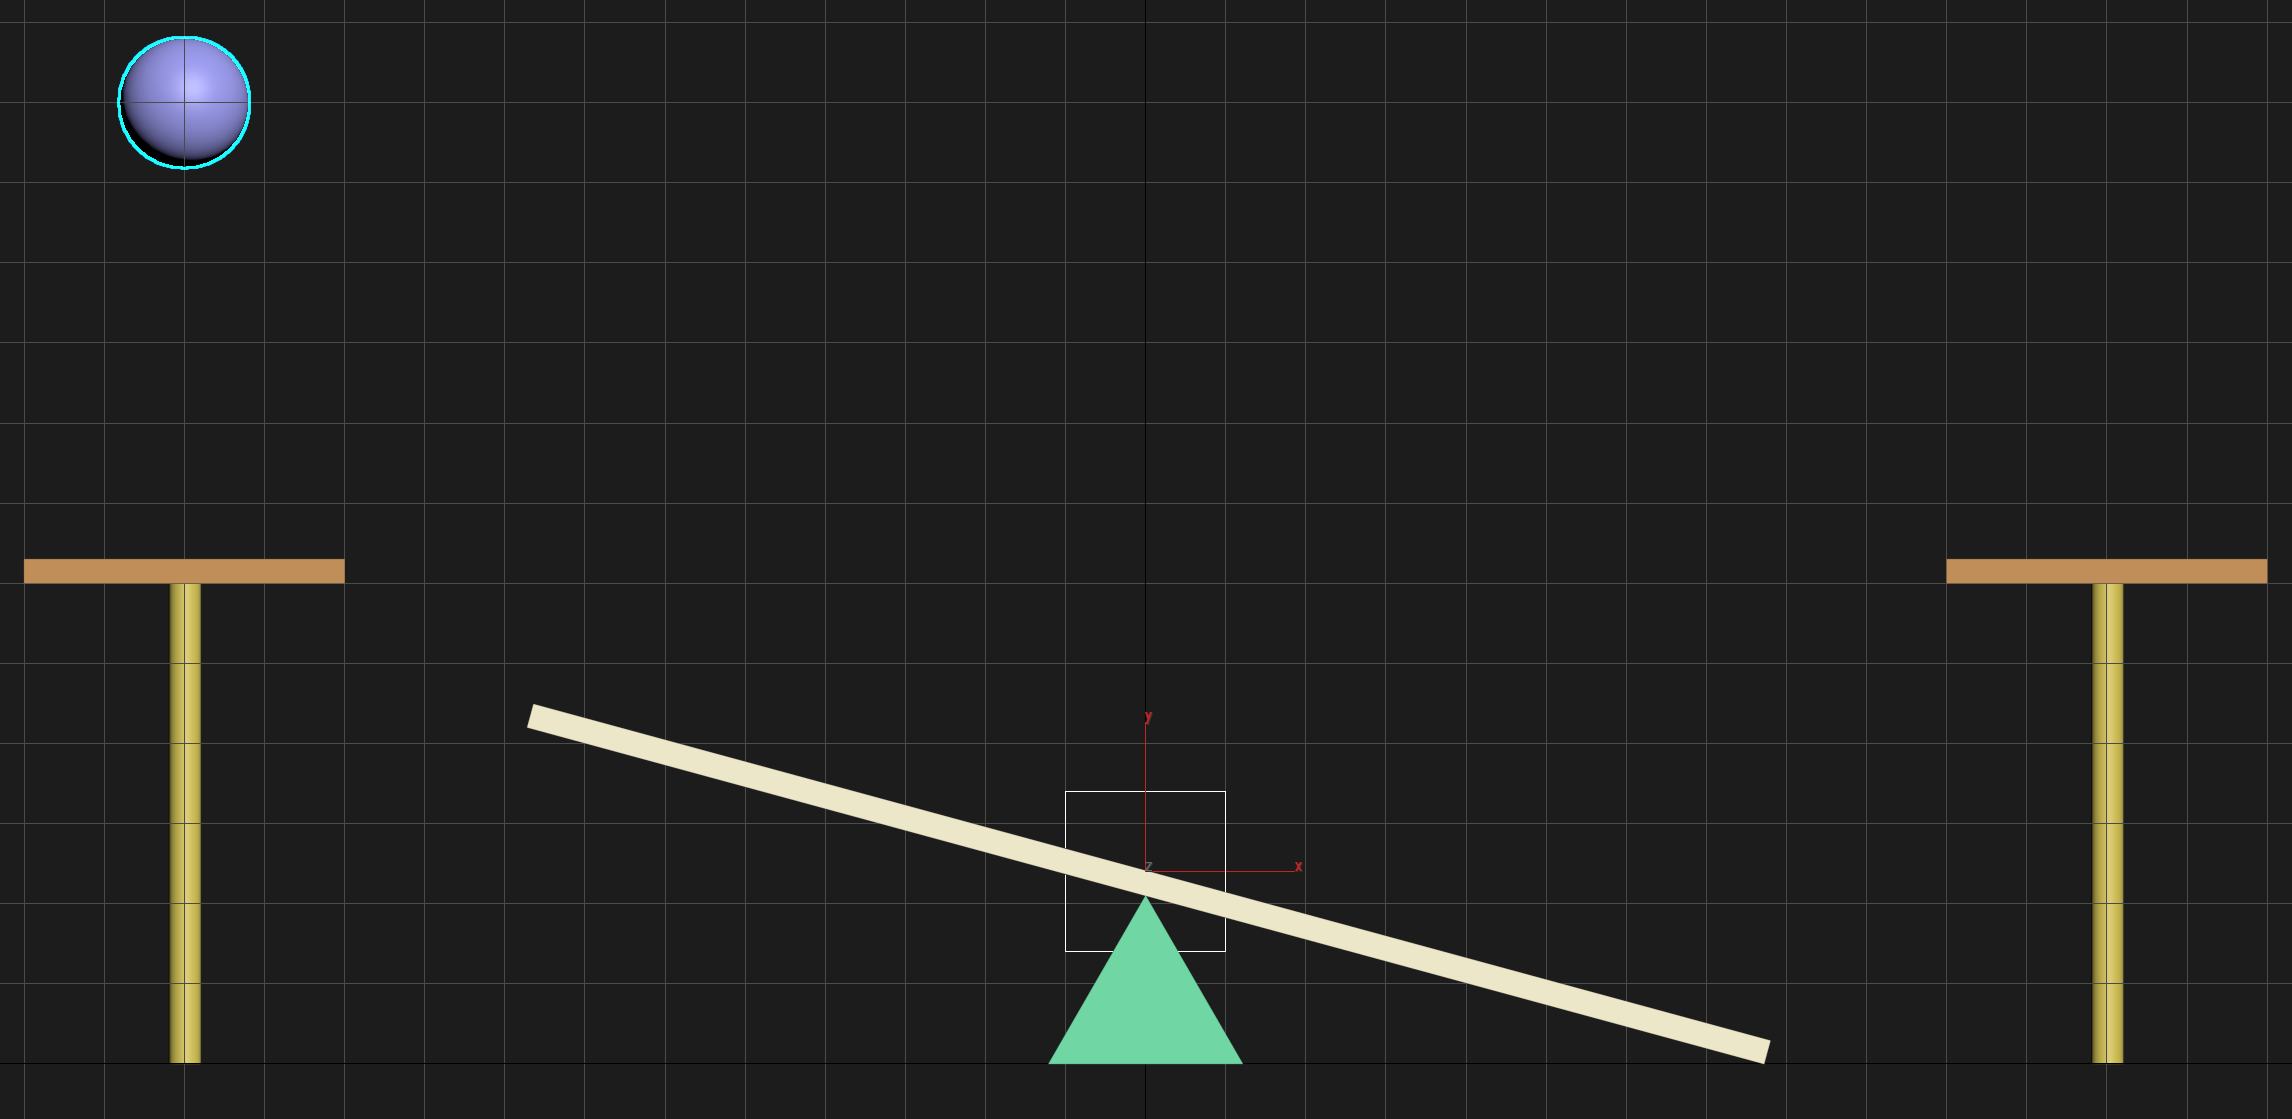
\includegraphics[width=0.7\textwidth]{imagenes/misc/PLDummy.png}
%    \caption{Pelota izquierda junto a su \textit{Dummy}.}
% \end{figure}


\newpage
\subsection{Pelota de la derecha}
De nuevo, como he dicho al principio de esta sección, he utilizado un \textit{Dummy} para realizar la animación del balanceo de manera correcta y algo más fácil que animarlo manualmente.

\bigskip

Por tanto, los \textit{keyframes} de la pelota de la derecha son:

\begin{itemize}
    \item \textbf{Instante 0: }La pelota se encuentra sobre la superficie del trampolín. Este instante solo es una extensión para que la animación ping-pong funcione correctamente y al mismo tiempo.
    \item \textbf{Instante 92: }Exactamente igual que el instante anterior.
    \item \textbf{Instante 102: }La pelota se encuentra sobre el punto más alto de la trayectoria hacia la base.
    \item \textbf{Instante 112: }La pelota ha acabado de realizar la trayectoria y se encuentra sobre la superficie de la base.
    \item \textbf{Instante 124: }La pelota se encuentra en el aire porque ha realizado un rebote.
    \item \textbf{Instante 136: }Ahora la pelota ha caído al suelo.
    \item \textbf{Instante 150: }Finalmente, la pelota da otro rebote y se encuentra en el aire de nuevo.
\end{itemize}

\bigskip

Las curvas de animación es:

\begin{figure}[H]
    \centering
    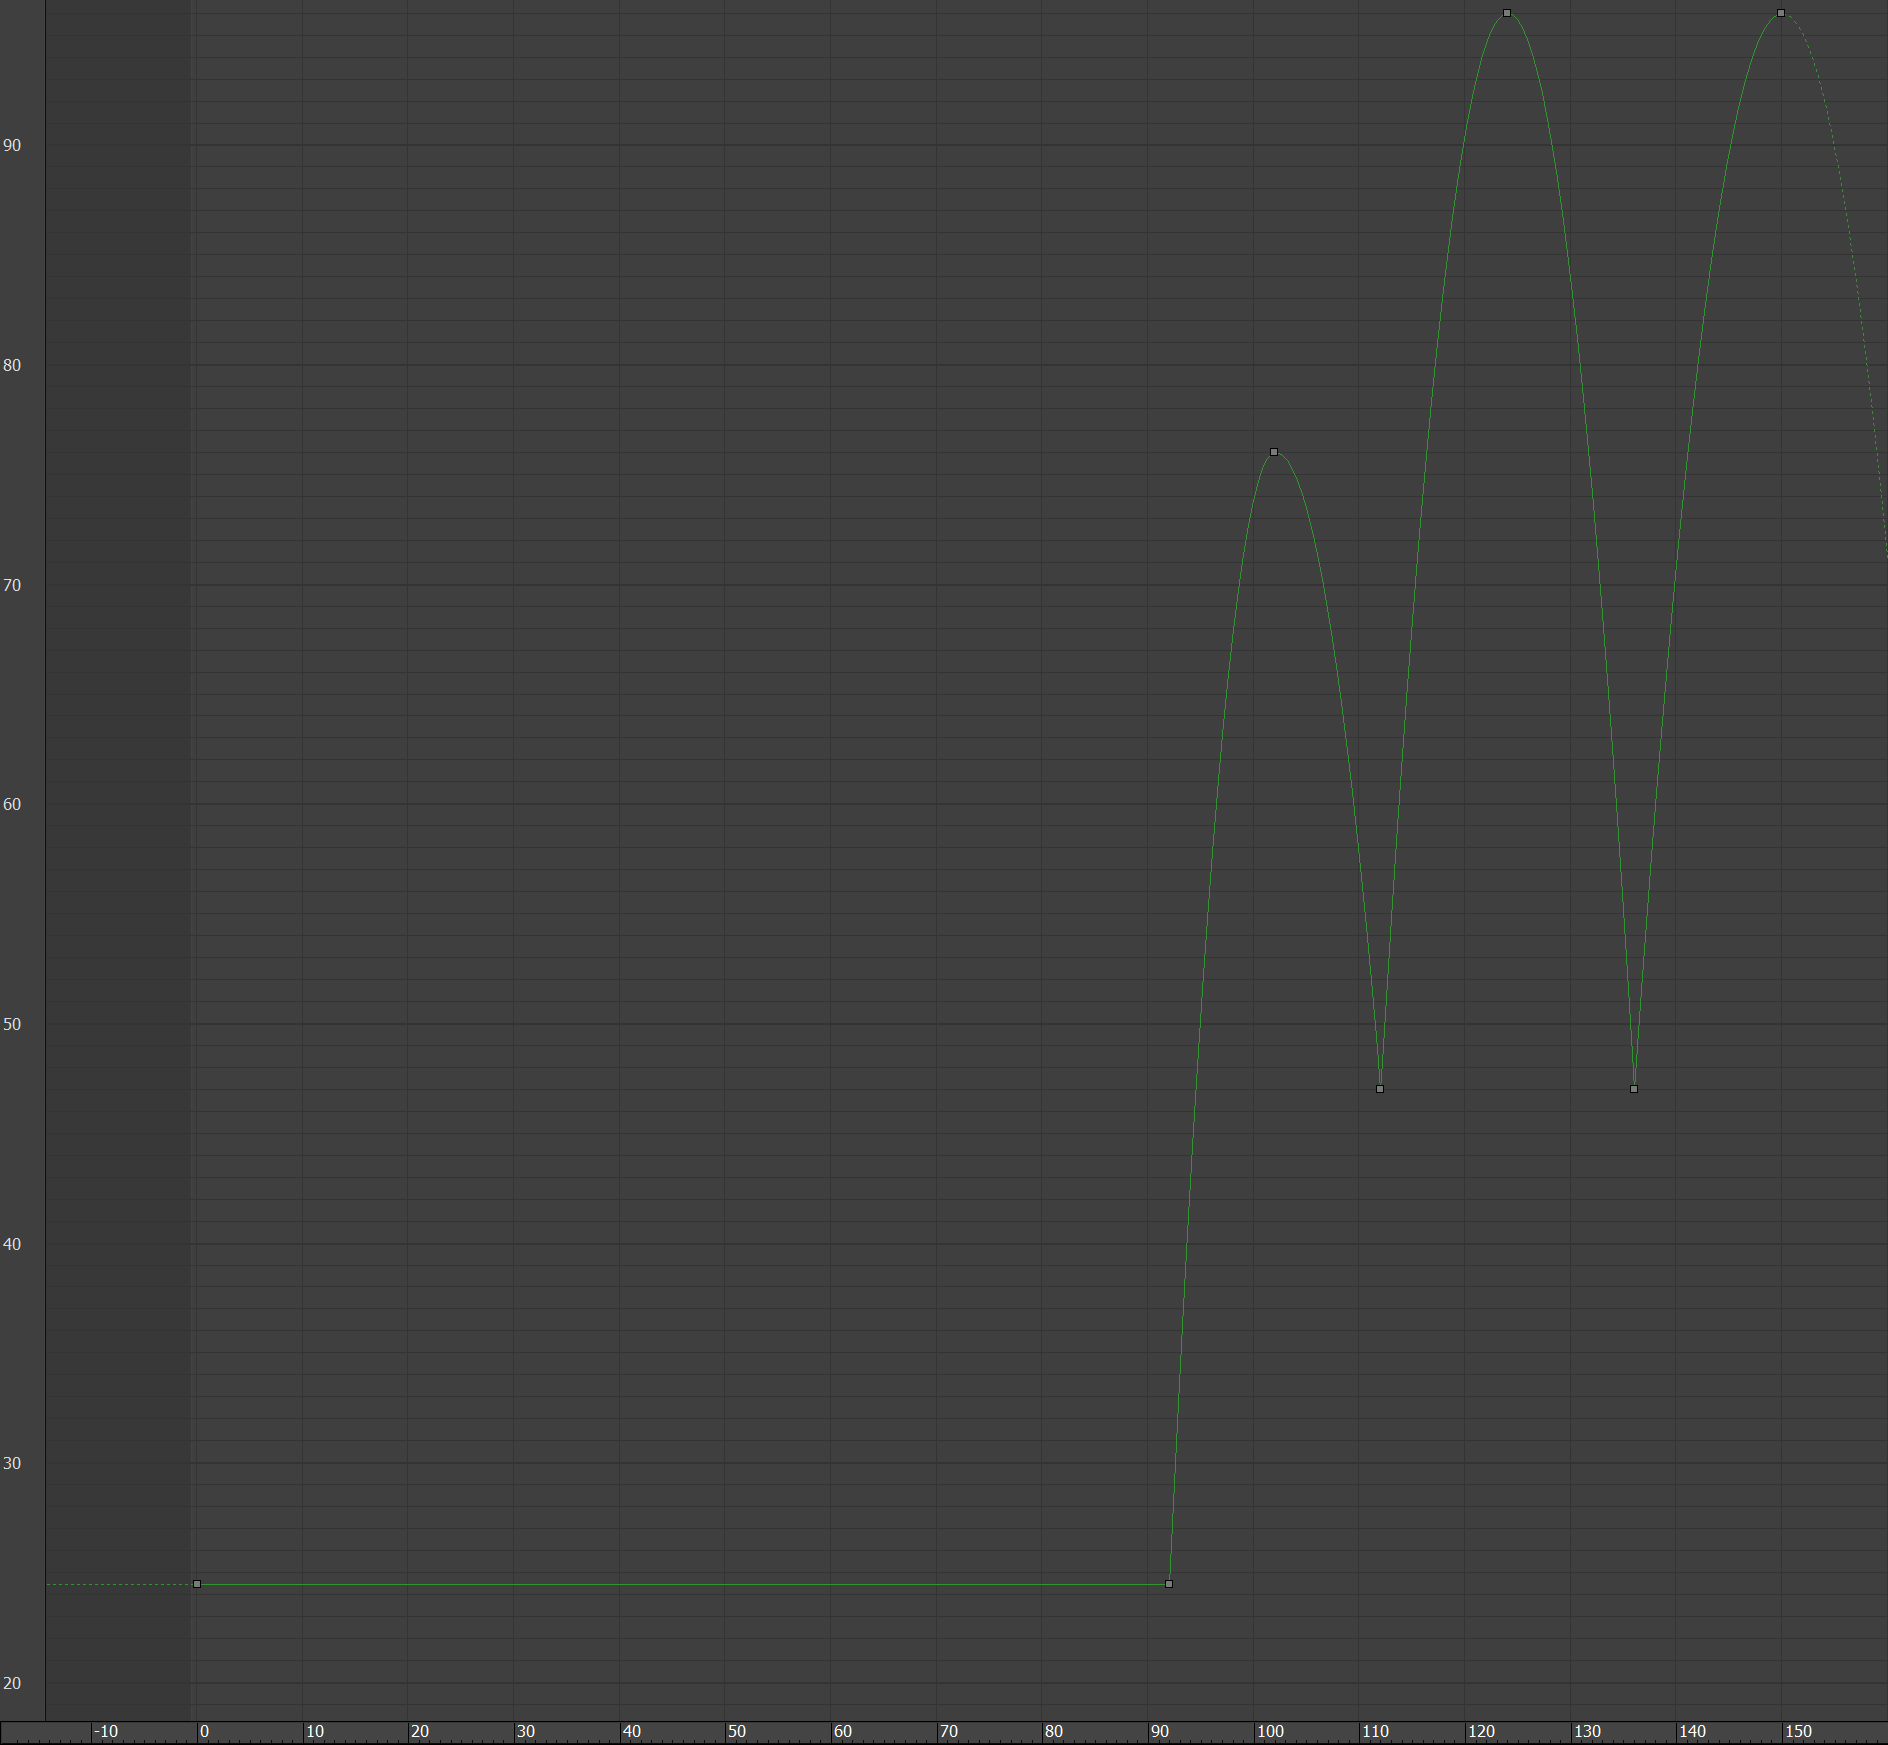
\includegraphics[width=0.6\textwidth]{imagenes/curvas/PR/pelota/green.png}
    \caption{Curva que representa la posición en el eje Y con respecto el tiempo.}
 \end{figure}

 Al igual que con la pelota de la izquierda, debido al \textit{Dummy} el eje Z pasa a ser el eje Y, pero en coordenadas del mundo sigue siendo el Z. Además, ocurre exactamente igual que en la pelota de la izquierda, se utilizan parábolas para simular los efectos de la gravedad sobre la pelota y que produzca un resultado natural, tanto en la trayectoria como en las subidas y caídas.

 \begin{figure}[H]
    \centering
    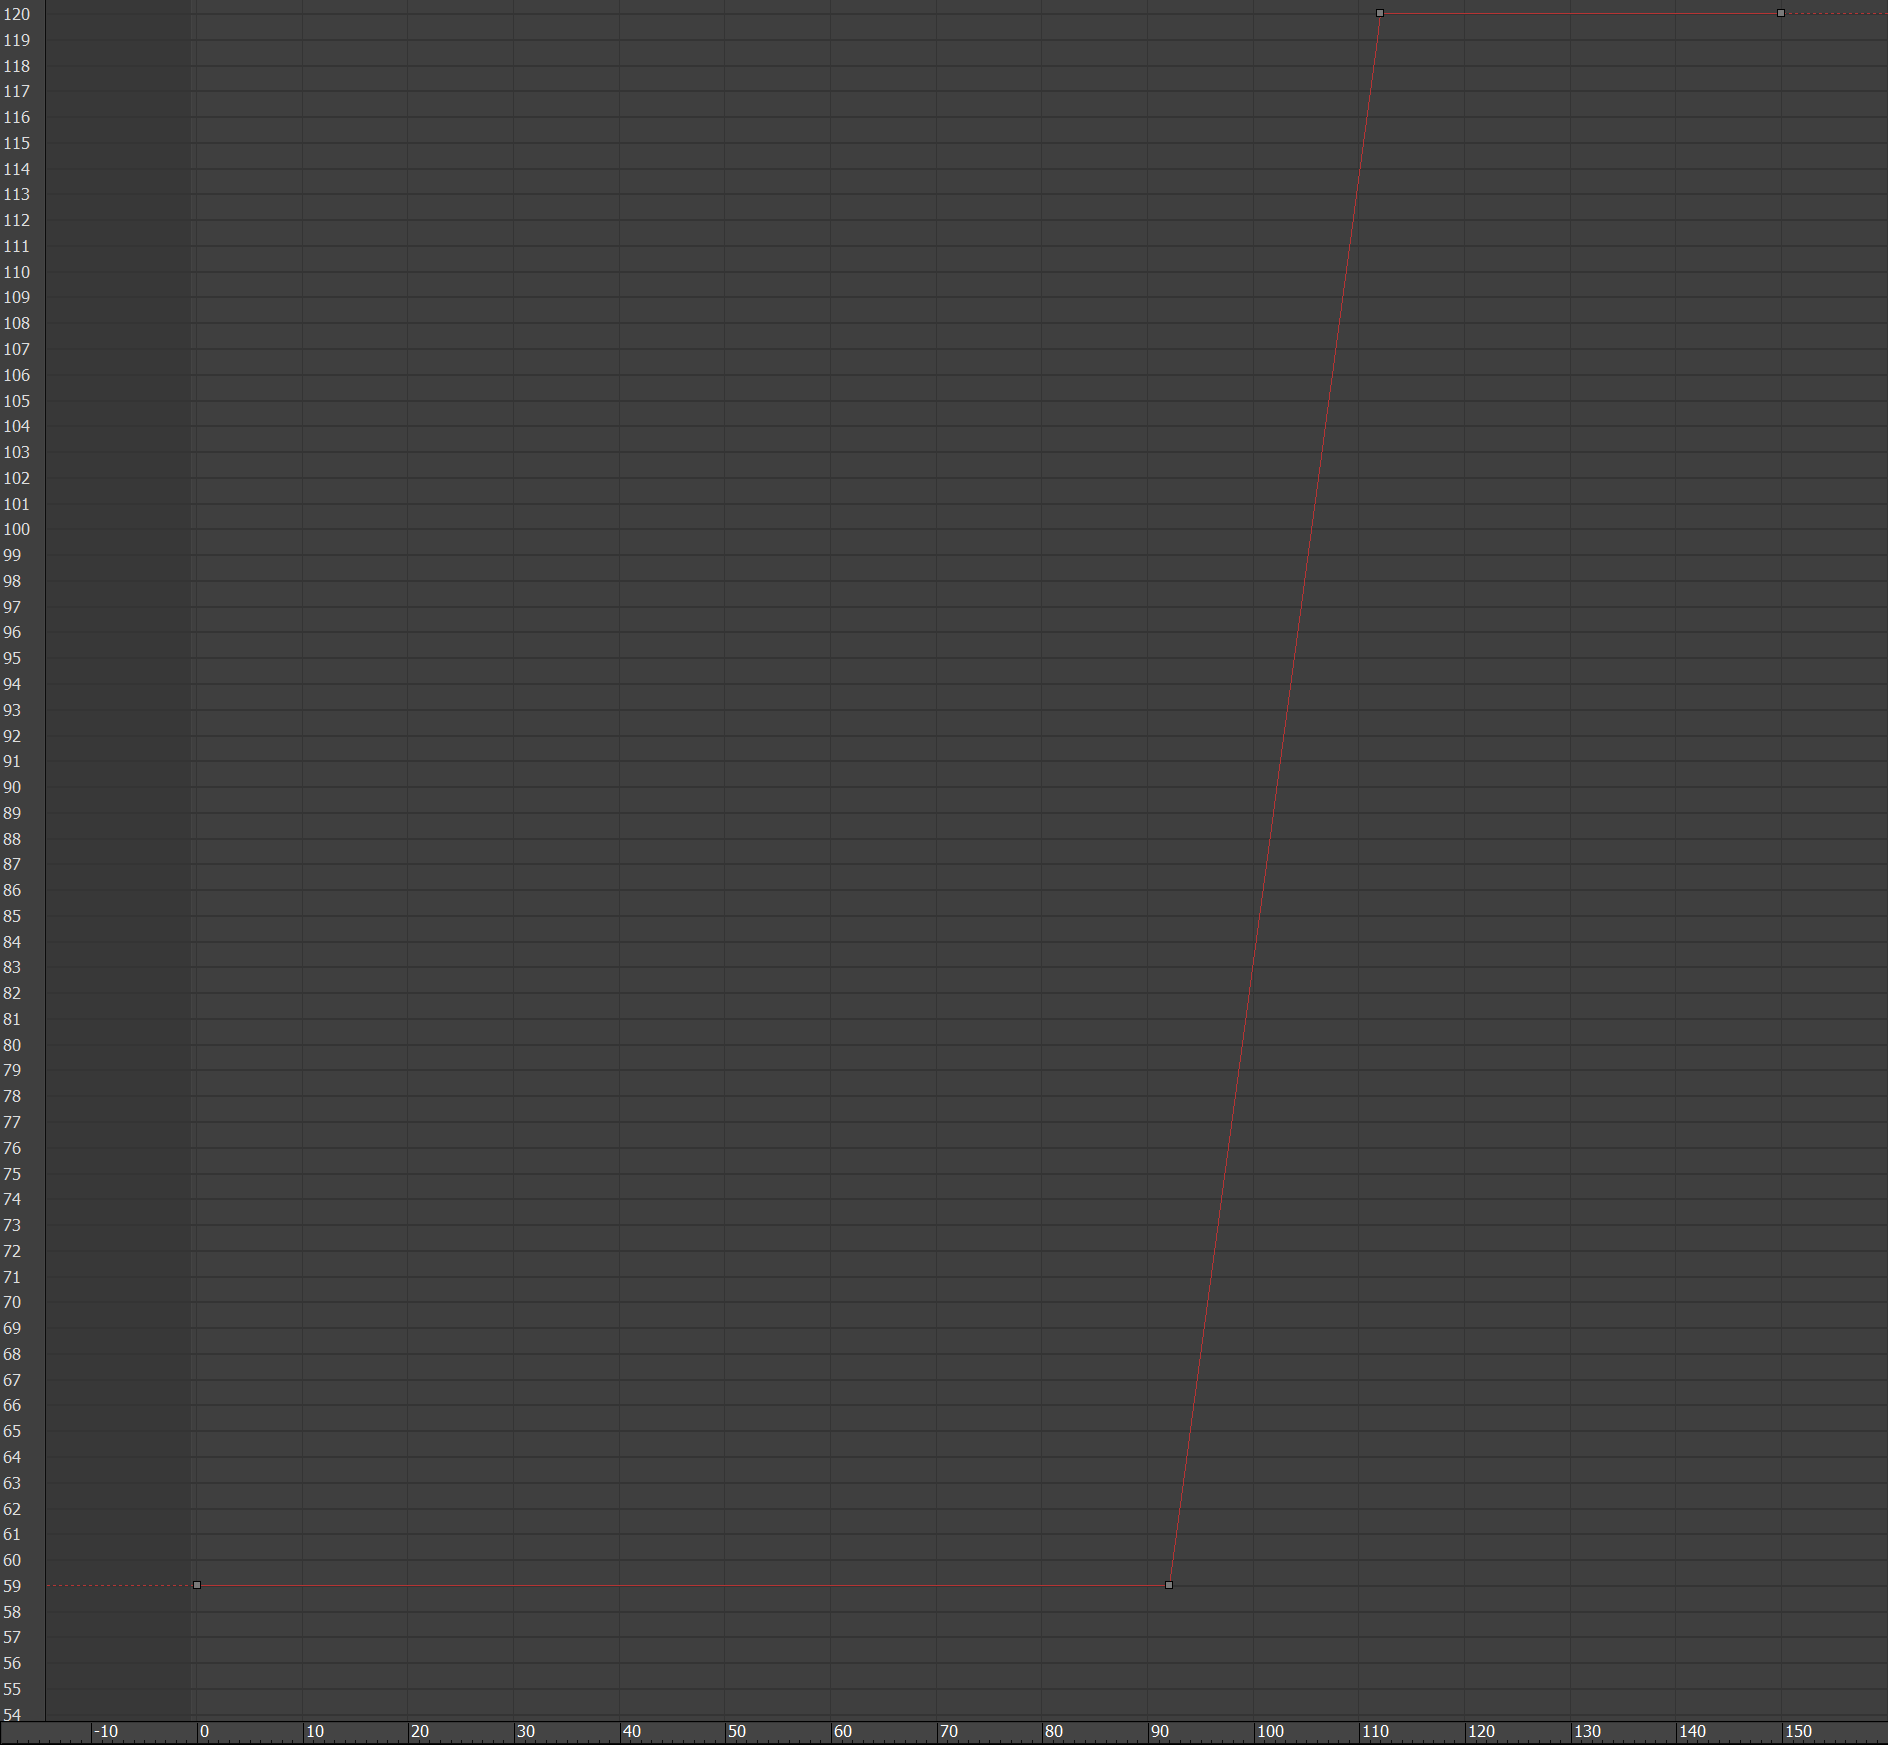
\includegraphics[width=0.6\textwidth]{imagenes/curvas/PR/pelota/red.png}
    \caption{Curva que representa la posición en el eje X con respecto el tiempo.}
 \end{figure}

Esta curva representa la posición en el eje X con respecto al tiempo. Ocurre de manera similar que con la pelota izquierda, he utilizado una función lineal porque era la que me parecía más realista.

\bigskip

Mientras que los \textit{keyframes} para su \textit{Dummy} son:

\begin{itemize}
    \item \textbf{Instante 0: }El \textit{Dummy} se encuentra rotado para que la pelota se encuentre sobre el trampolín. Al igual que con la pelota, se debe hacer para que la animación inversa se haga al mismo tiempo.
    \item \textbf{Instante 58: }No ha habido cambios en la animación, es igual que el instante anterior.
    \item \textbf{Instante 92: }Ahora el \textit{Dummy} se encuentra rotado en la posición original; es decir, sin ninguna rotación aplicada para que la trayectoria de la pelota sea correcta.
    \item \textbf{Instante 150: }Ningún cambio realizado, solo es para que la animación inversa comience a la misma vez.
\end{itemize}

\newpage

La curva de animación para el \textit{Dummy} es:

\begin{figure}[H]
    \centering
    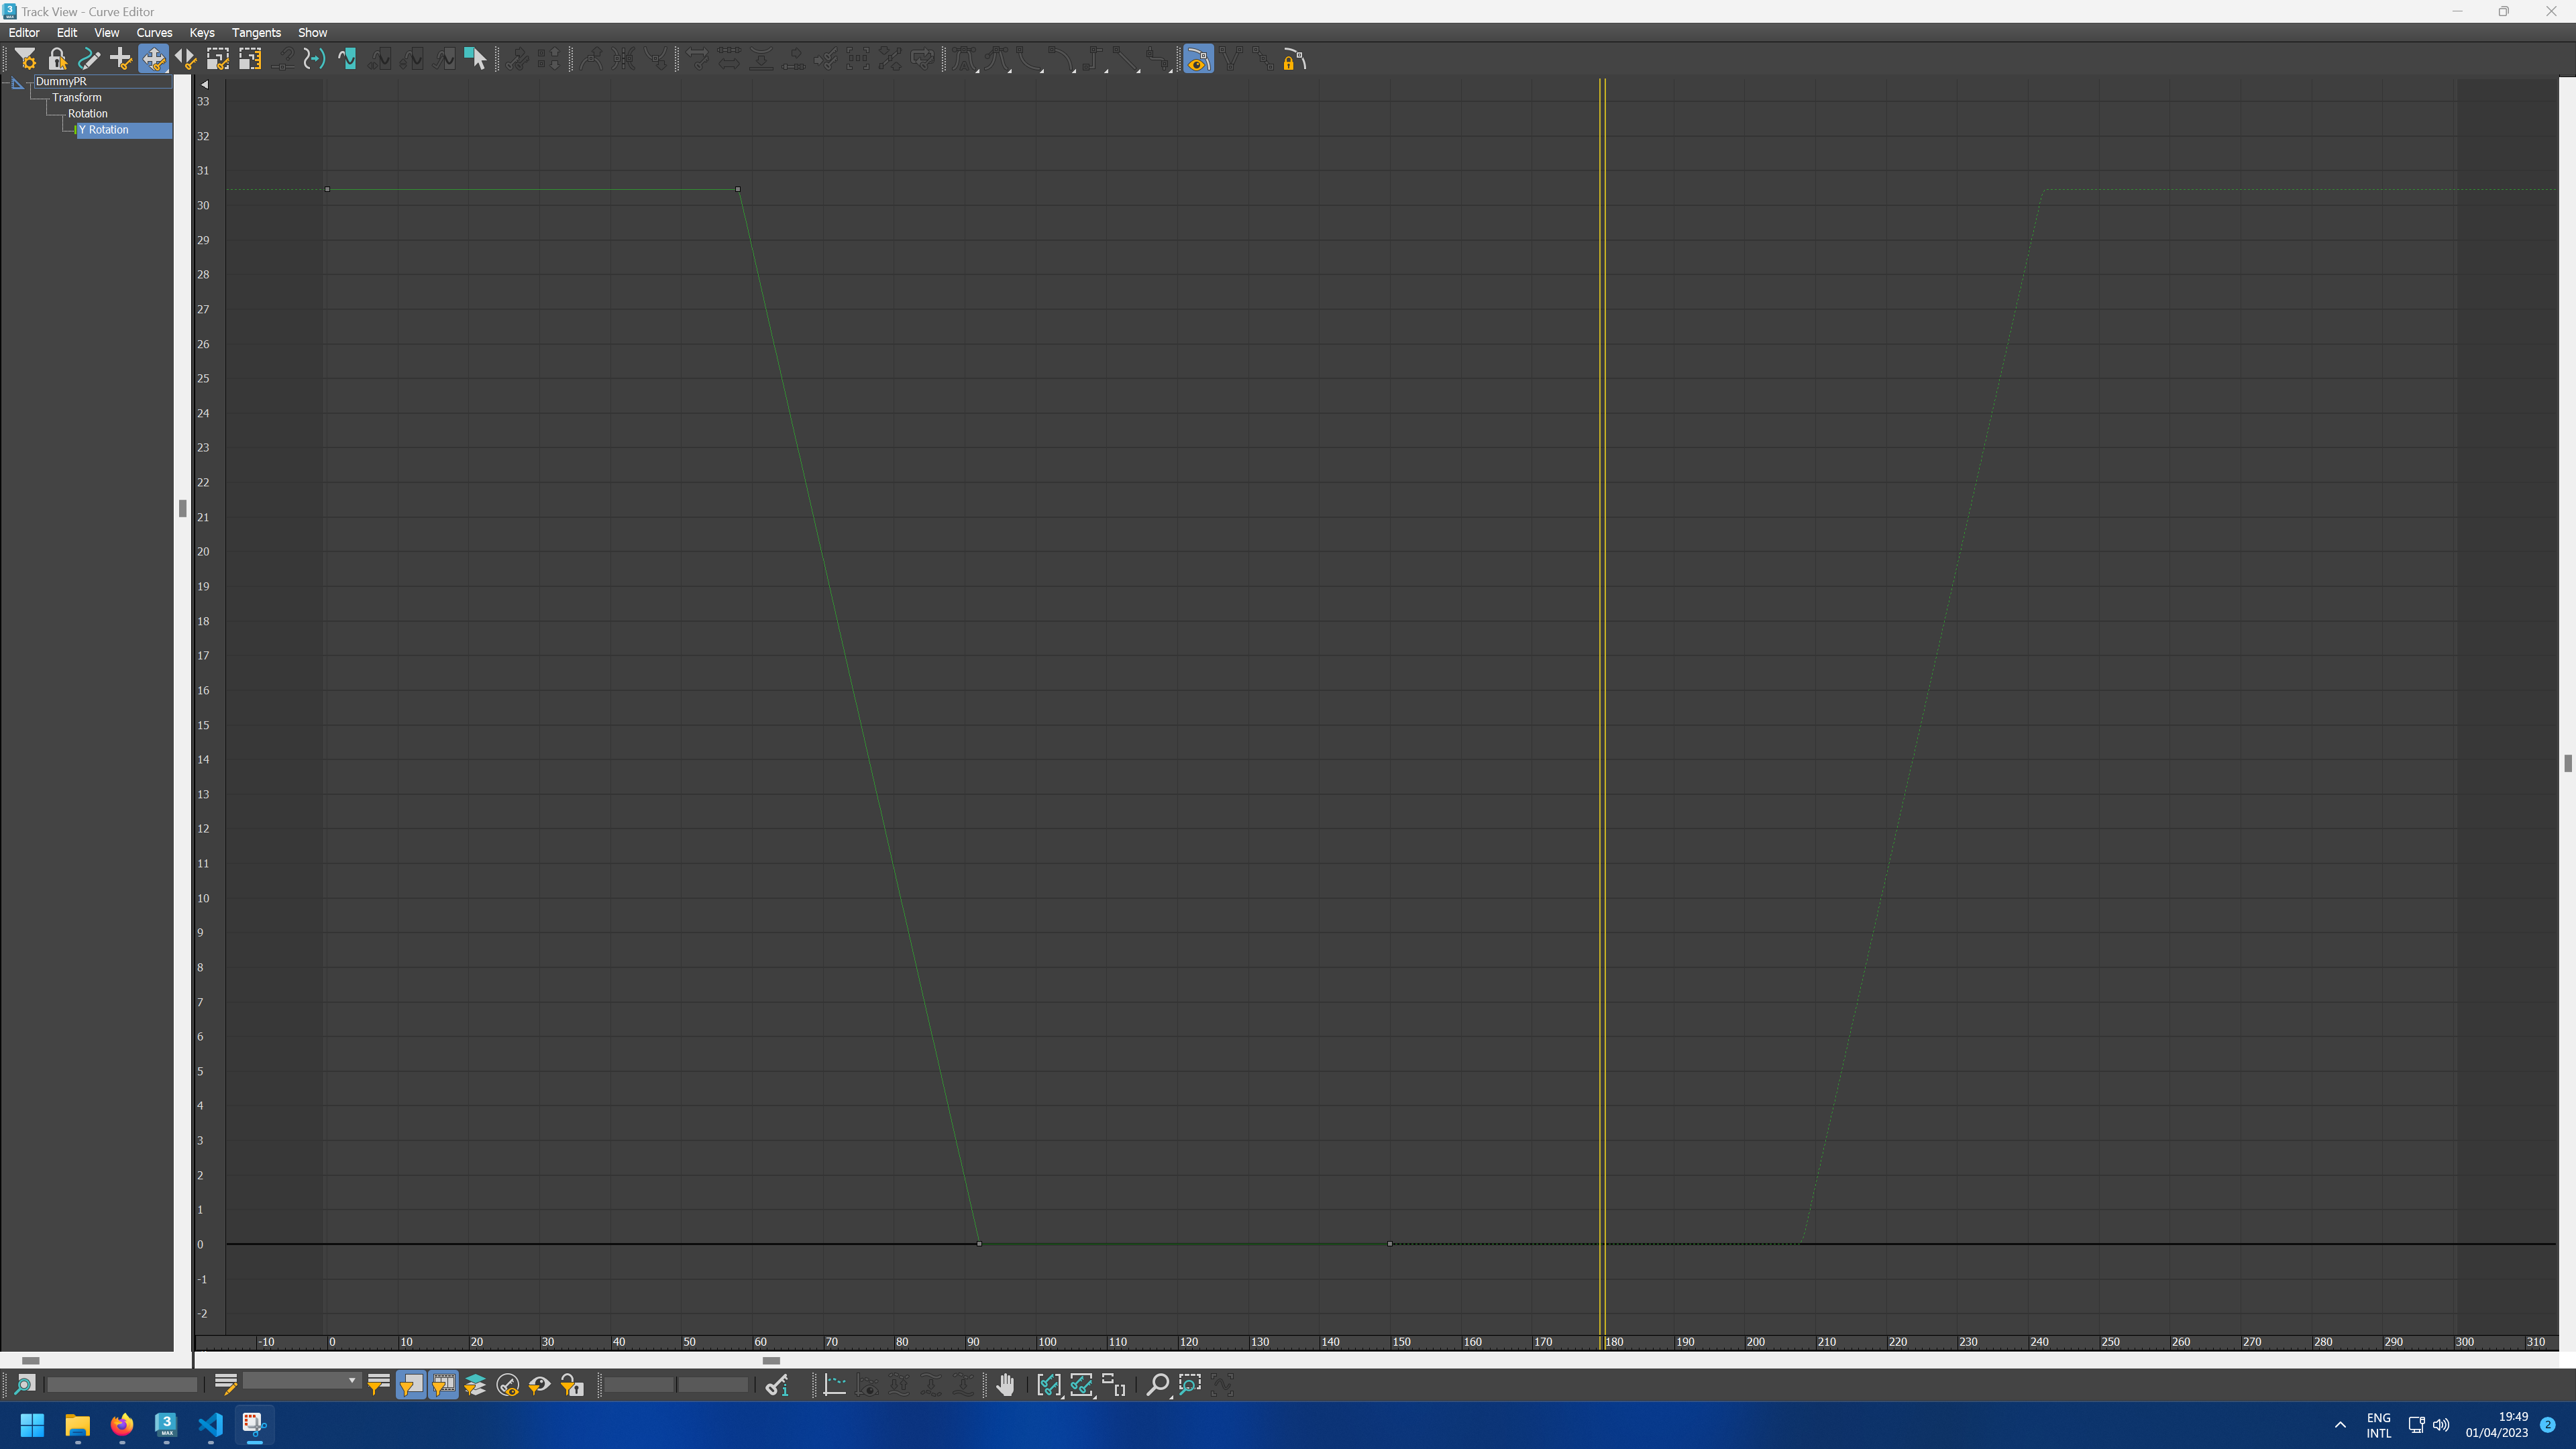
\includegraphics[width=0.6\textwidth]{imagenes/curvas/PR/dummy/green.png}
    \caption{Curva que representa la rotación en el eje Y con respecto el tiempo.}
 \end{figure}

De nuevo, ocurre de manera similar que con el \textit{Dummy} de la otra pelota. La curva es lineal, ya que la pelota le transfiere al trampolín toda la energía potencial que tenía, haciendo que no tenga tiempo de acelerar y se ponga a la velocidad máxima directamente.

\bigskip

Además, esta pelota sigue el mismo espaciado en los \textit{keyframes} que la otra, pero comenzando desde el instante 150 y hacia la izquierda; es decir, es como si fuera un ``reflejo'' de la otra. Esto resultará en que la pelota comience sobre el trampolín y acabe dando saltos sobre la plataforma, así se puede repetir la animación inversa de manera fluida.

\bigskip

% La pelota y su \textit{Dummy} se encuentran en la escena de la siguiente forma:

% \begin{figure}[H]
%    \centering
%    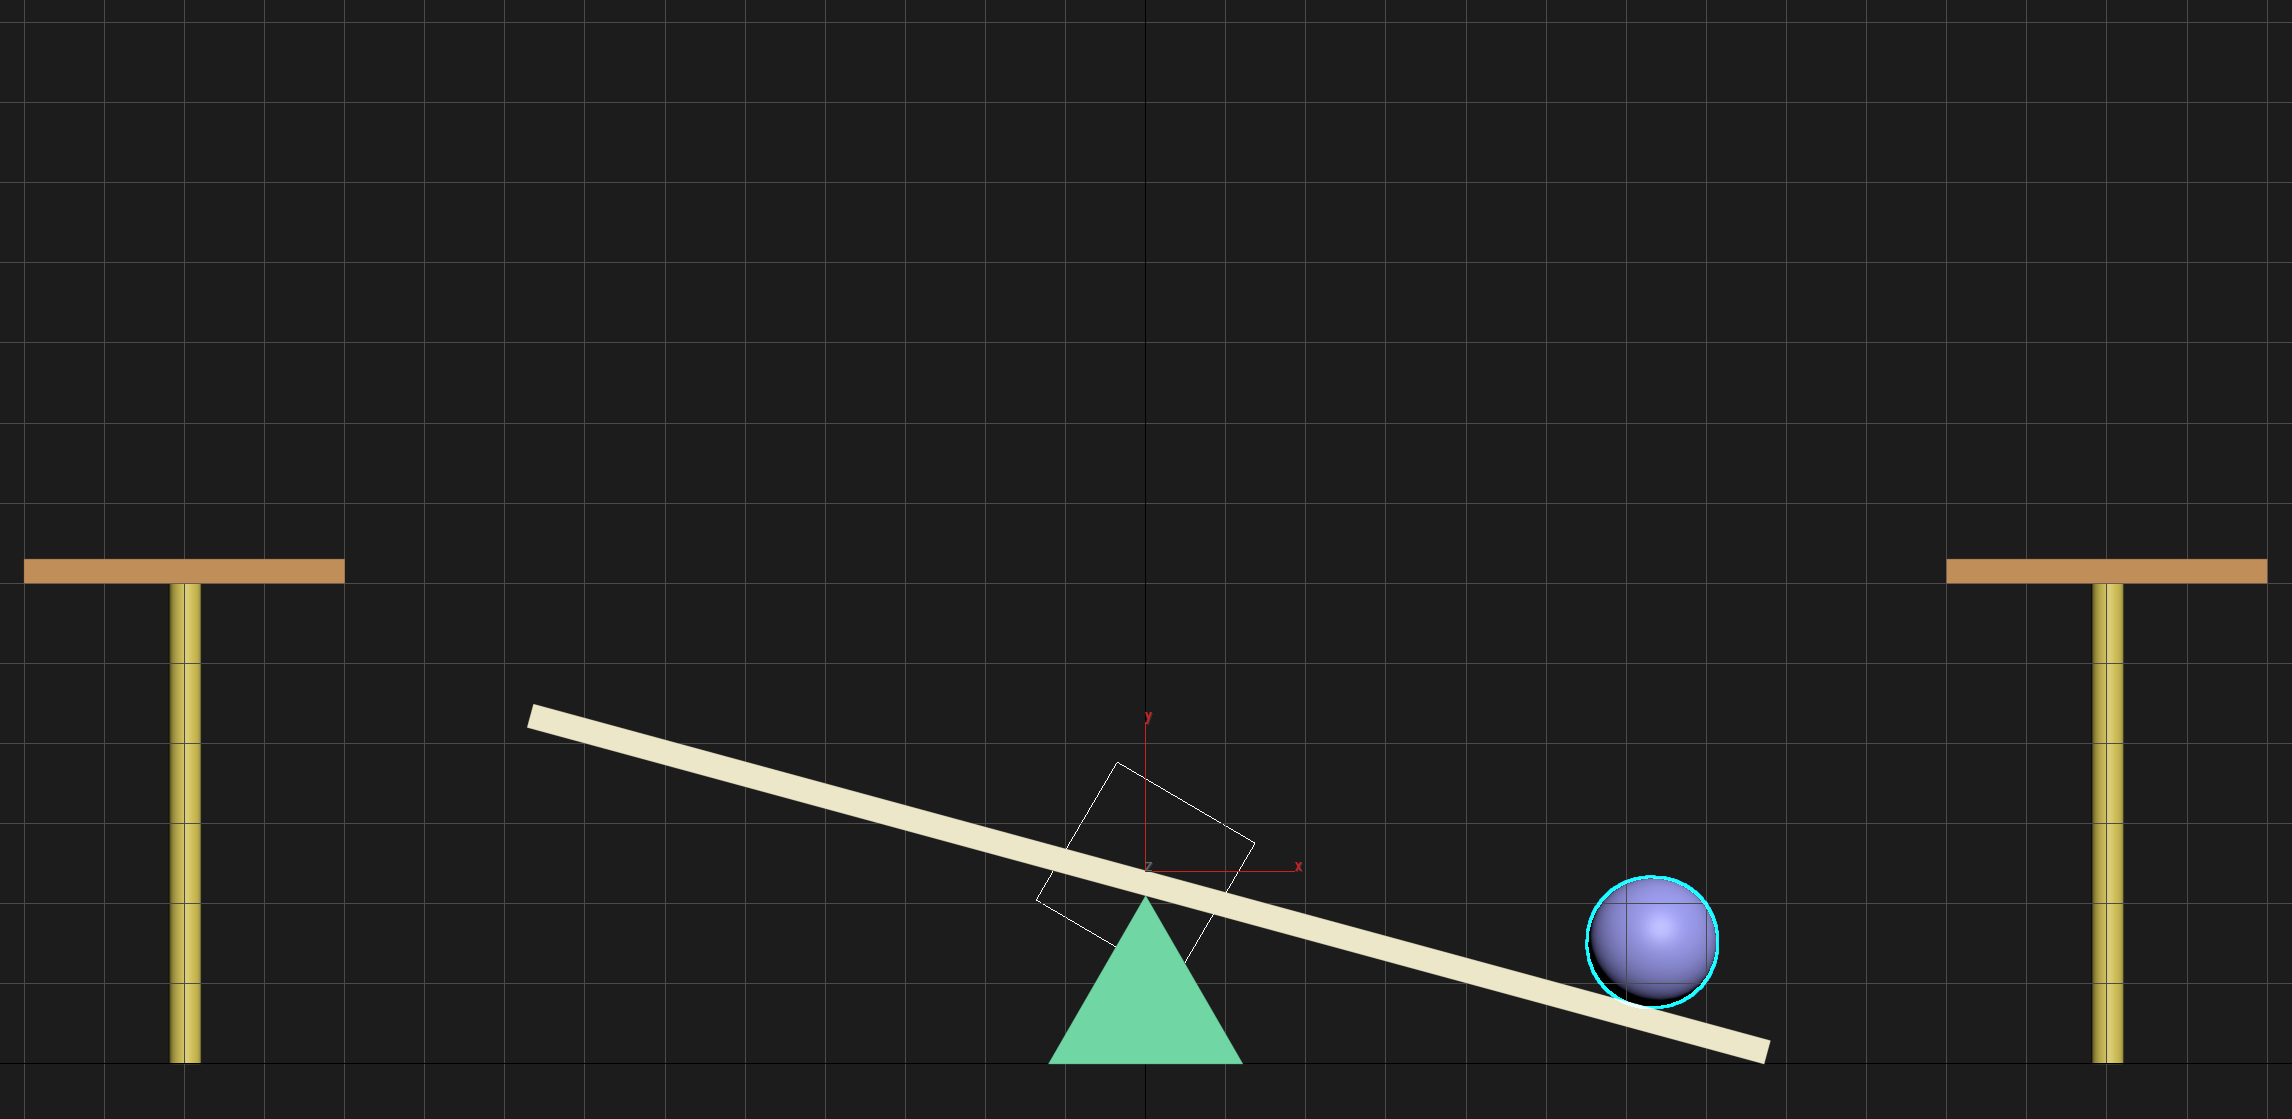
\includegraphics[width=0.7\textwidth]{imagenes/misc/PRDummy.png}
%    \caption{Pelota derecha junto a su \textit{Dummy}.}
% \end{figure}

\newpage
\subsection{Trampolín}
Para realizar el giro de la curva del trampolín es necesario sincronizar los instantes iniciales y finales de los \textit{dummies} de las pelotas, para que giren conjuntamente. Asimismo, como he dicho al principio de la sección, es necesario mover el pivote de la base justo en la unión del punto de apoyo, para que gire de manera correcta.

\bigskip

Los \textit{keyframes} para realizar la animación del trampolín son los siguientes:

\begin{itemize}
    \item \textbf{Instante 0: }Se encuentra girado hacia la derecha, con la pelota derecha sobre el trampolín. Como se ha dicho anteriormente, este instante es para sincronizar las animaciones con la parte en la que se realiza de forma inversa.
    \item \textbf{Instante 58: }Exactamente igual que el anterior instante.
    \item \textbf{Instante 92: }El trampolín ahora se encuentra girado hacia el otro lado debido a la energía que le transfiere la pelota izquierda.
    \item \textbf{Instante 150: }No varía nada de la animación con respecto al instante anterior. Ocurre exactamente igual que en el instante 0.
\end{itemize}

\bigskip

Y la curva de animación es:

\begin{figure}[H]
    \centering
    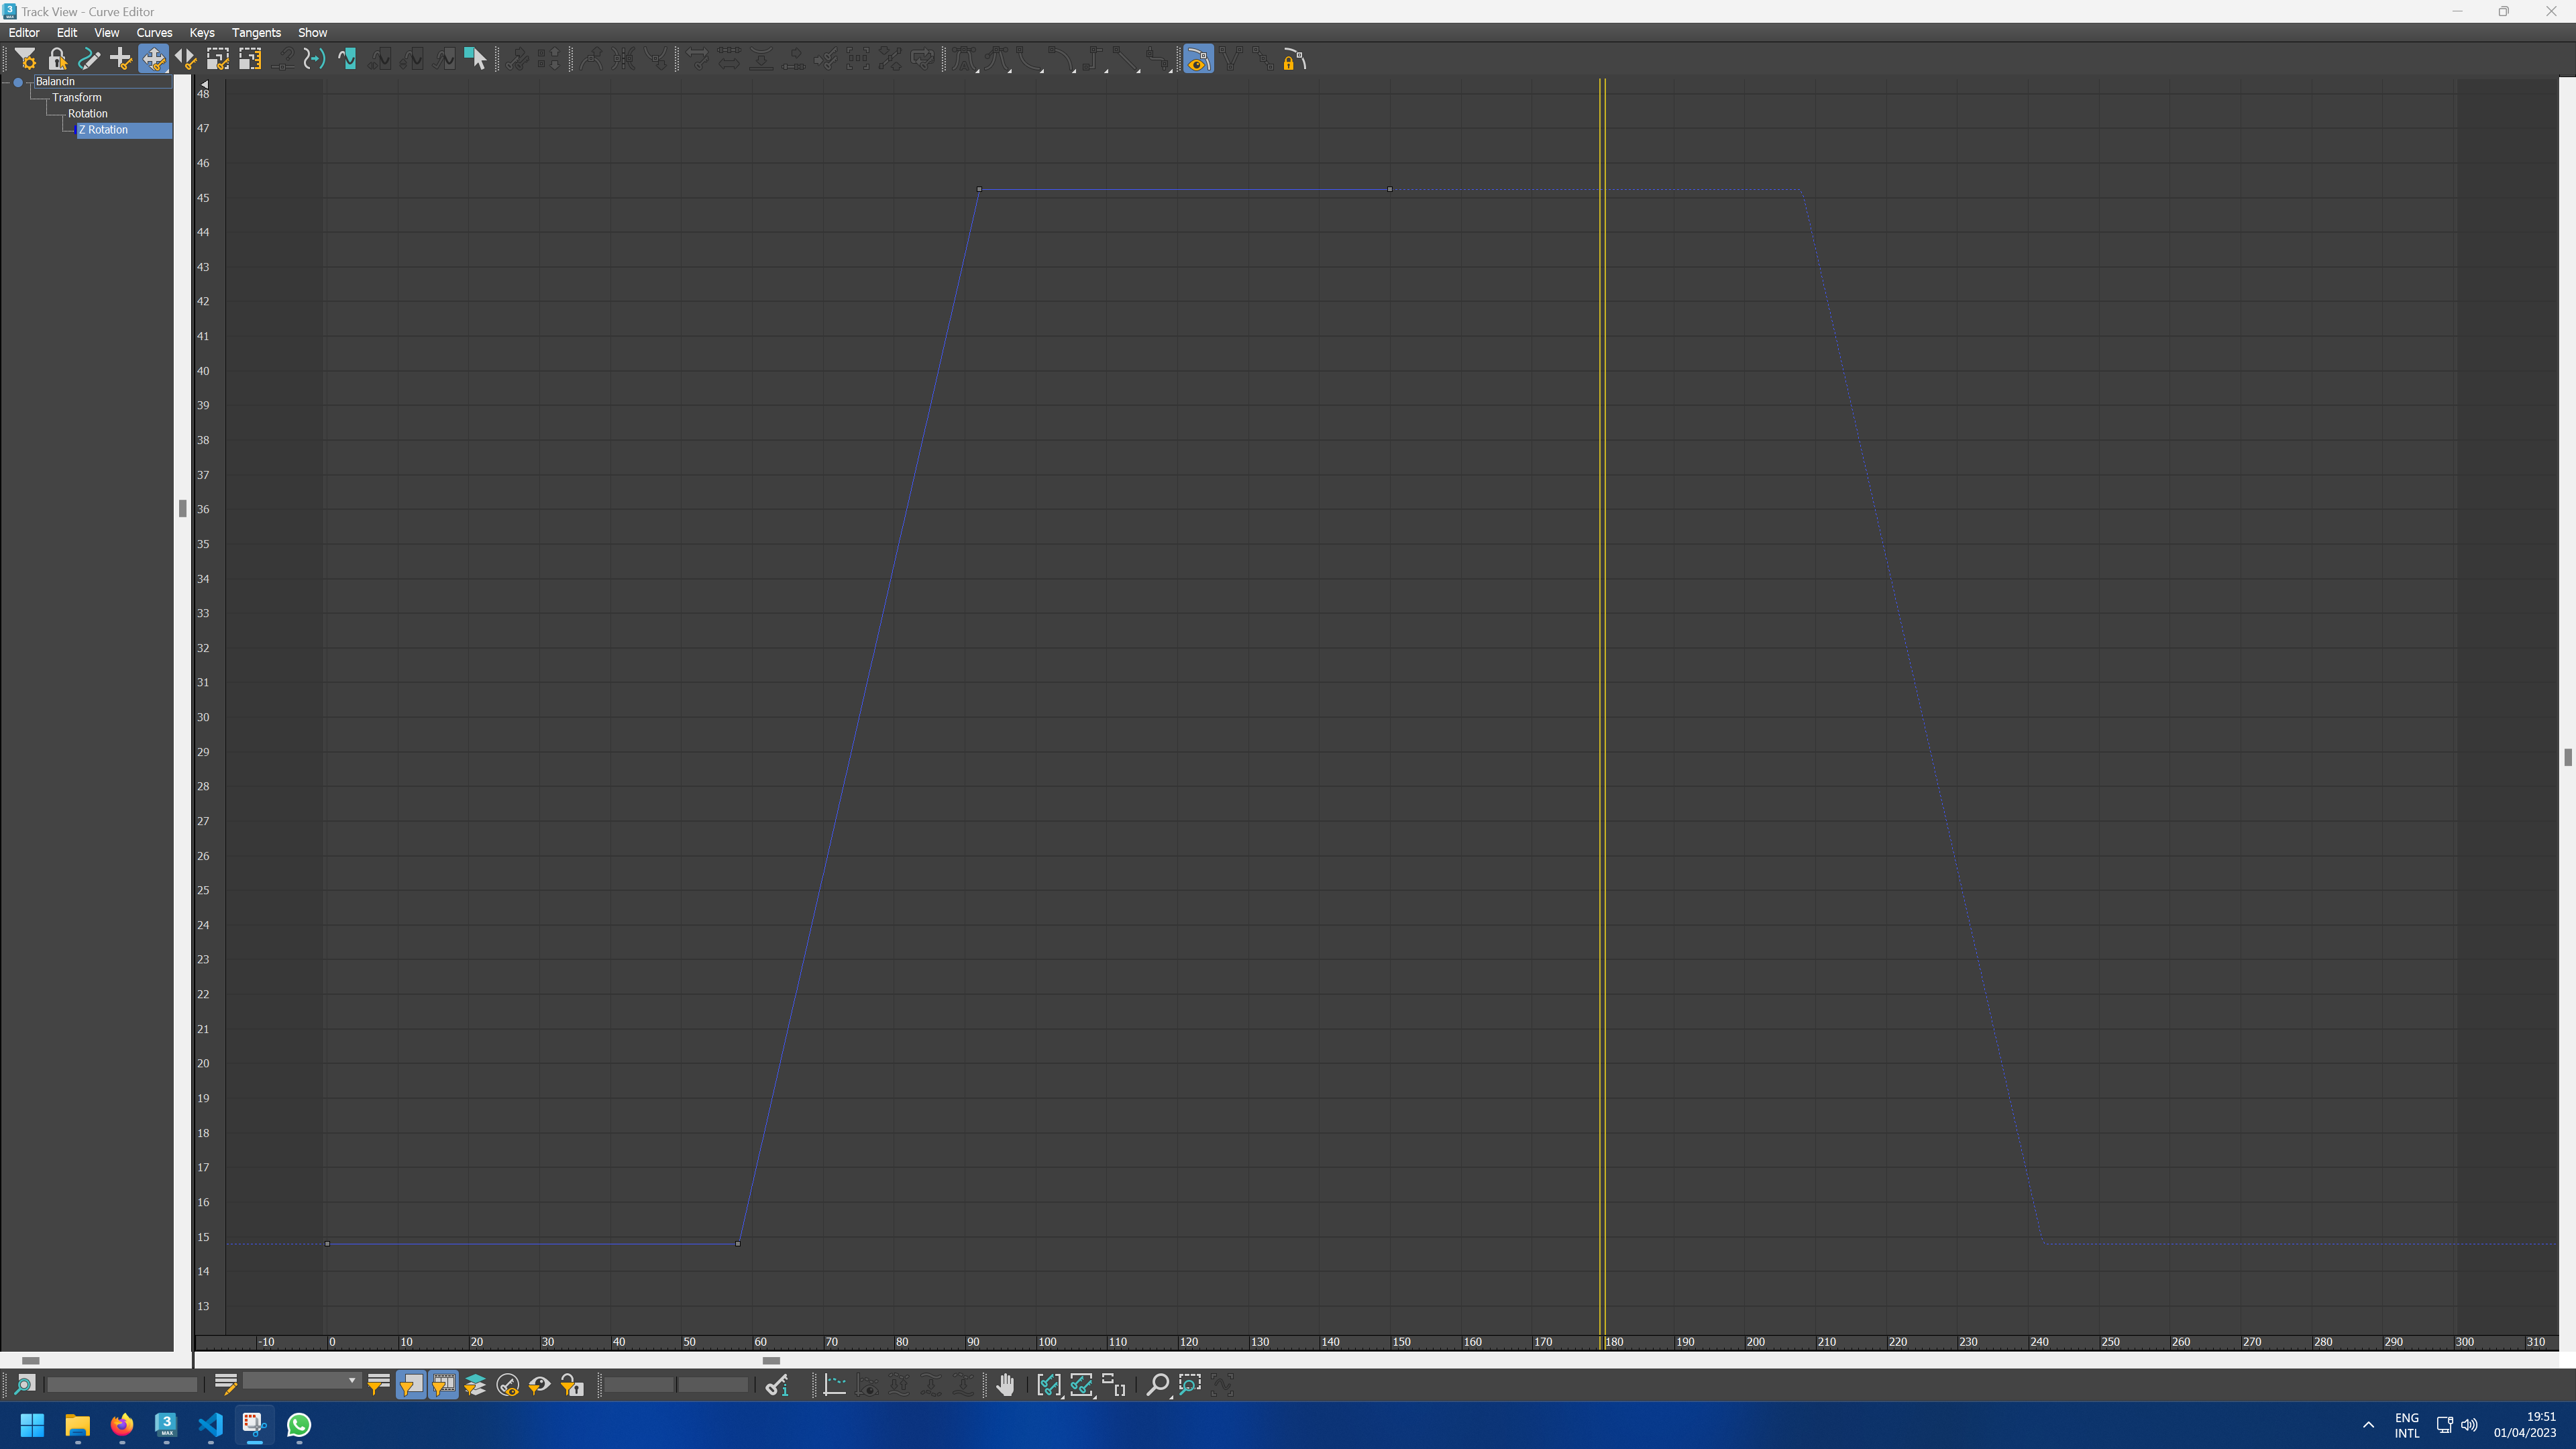
\includegraphics[width=0.6\textwidth]{imagenes/curvas/Trampolin/blue.png}
    \caption{Curva que representa la rotación en el eje Z con respecto al tiempo.}
 \end{figure}

 Al igual que las pelotas, como el balancín es hijo del punto de apoyo, la rotación realmente se ve reflejada en el eje Y en coordenadas del mundo, ya que el padre actúa de manera similar a los \textit{dummies}. Al igual que estos, el trampolín utiliza una curva lineal, ya que la energía potencial de la pelota que se encuentra en el aire, al tocarlo se la transfiere, sin la posibilidad de que acelere poco a poco.